
%\newtheorem{definition}[subsection]{Definition}
%\newtheorem{example}[subsection]{Example}
\newtheorem{cor}[subsection]{Corollary}
\newtheorem{pro}[subsection]{Proposition}
\newtheorem{theo}[subsection]{Theorem}
\newtheorem{lem}[subsection]{Lemma}
%\newtheorem{rem}[subsection]{Remark}

\definecolor{main}{HTML}{5989cf}    % setting main color to be used
\definecolor{sub}{HTML}{cde4ff}     % setting sub color to be used

\tcbset{
    sharp corners,
    colback = white,
    before skip = 0.2cm,    % add extra space before the box
    after skip = 0.5cm      % add extra space after the box
}                           % setting global options for tcolorbox

% You can copy any following box you like to your code.
\newtcolorbox{boxA}{
    fontupper = \bf,
    boxrule = 1.5pt,
    colframe = black % frame color
}

\newtcolorbox{boxB}{
    fontupper = \bf\color{main}, % font color
    boxrule = 1.5pt,
    colframe = main,
    rounded corners,
    arc = 5pt   % corners roundness
}
\newtcolorbox{boxC}{
    colback = sub, % background color
    boxrule = 0pt  % no borders
}

\newtcolorbox{boxD}{
    colback = sub, 
    colframe = main, 
    boxrule = 0pt, 
    toprule = 3pt, % top rule weight
    bottomrule = 3pt % bottom rule weight
}

\hypersetup{
    colorlinks=true,
    linkcolor=blue,
    filecolor=magenta,      
    urlcolor=cyan,
    pdftitle={Overleaf Example},
    pdfpagemode=FullScreen,
    }

\urlstyle{same}


\coursetitle{\mtthreeiii}{MT303}
\developers{Wyclife Rao}
\reviewers{Dr Irene Sitawa}
\modulenumber{8}
\modulename{Initial-Value Problems for Ordinary Differential Equations II}

% courses
\thispagestyle{empty}
\begin{tikzpicture}[overlay,remember picture,font=\sffamily\bfseries]
 \draw[ultra thick,c4,name path=big arc] ([xshift=-2mm]current page.north) arc(150:285:11) coordinate[pos=0.225] (x0);
 \begin{scope}
  \clip ([xshift=-2mm]current page.north) arc(150:285:11) --(current page.north east);
  \fill[c4!50,opacity=0.25] ([xshift=4.55cm]x0) circle (4.55);
  \fill[c4!50,opacity=0.25] ([xshift=3.4cm]x0) circle (3.4);
  \fill[c4!50,opacity=0.25] ([xshift=2.25cm]x0) circle (2.25);
  \draw[ultra thick,c4!50] (x0) arc(-90:30:6.5);
  \draw[ultra thick,c4] (x0) arc(90:-30:8.75);
  \draw[ultra thick,c4!50,name path=arc1] (x0) arc(90:-90:4.675);
  \draw[ultra thick,c4!50] (x0) arc(90:-90:2.875);
  \path[name intersections={of=big arc and arc1,by=x1}];
  \draw[ultra thick,c4,name path=arc2] (x1) arc(135:-20:4.75);
  \draw[ultra thick,c4!50] (x1) arc(135:-20:8.75);
  \path[name intersections={of=big arc and arc2,by={aux,x2}}];
  \draw[ultra thick,c4!50] (x2) arc(180:50:2.25);
 \end{scope} 
 \path[decoration={text along path,text color=c4,
                 raise = -2.8ex,
                 text  along path,
                 text = {},%|\sffamily\bfseries|02/18/2019
                 text align = center,
             },
             decorate
         ] ([xshift=-2mm]current page.north) arc(150:245:11);
 %
 \newcommand\add{4cm}
 \begin{scope}%[shift={(5,0)}]
  \path[clip,postaction={fill=c3}]
  ([xshift=2cm+\add,yshift=-8cm]current page.center) rectangle ++ (4.6,7.7);
  \draw[c5,ultra thick,fill=c2] ([xshift=0.5cm+\add,yshift=-8cm]current page.center)
   ([xshift=0.5cm+\add,yshift=-8cm]current page.center)  arc(180:60:2)
    |- ++ (-3,6) --cycle;
  \draw[ultra thick,c5] ([xshift=-1.5cm+\add,yshift=-8cm]current page.center) 
  arc(180:0:2);
  \draw[ultra thick,c5] ([xshift=0.5cm+\add,yshift=-8cm]current page.center) 
  arc(180:0:2);
  \draw[ultra thick,c5] ([xshift=2.5cm+\add,yshift=-8cm]current page.center) 
  arc(180:0:2);
  \draw[ultra thick,c5] ([xshift=4.5cm+\add,yshift=-8cm]current page.center) 
  arc(180:0:2);
  \fill[white] ([xshift=2.5cm+\add,yshift=-8cm]current page.center) +(60:2) circle(1.5mm)
  node[above
  right=0mm,text=c5!80!black]{$\rho:=\dfrac{1+\sqrt{-3}}{2}$};
 \end{scope}
 %
 \fill[c1] ([xshift=2cm+\add,yshift=-8cm]current page.center) rectangle ++ (-30.7,7.7);
 \node[text=white,anchor=west,scale=2.3,inner sep=0pt] at
 ([xshift=-10cm,yshift=-1.8cm]current page.center) {\color{ulabgold} LEARNING};
 \node[text=white,anchor=west,scale=5,inner sep=0pt] at
 ([xshift=-10cm,yshift=-3.25cm]current page.center) {MODULE \dpmdnumber};
 \node[text=white,anchor=west,scale=2.5,inner sep=0pt,text width=.4\textwidth] at
 ([xshift=-10cm,yshift=-6cm]current page.center) {\dpmdname};
 \node[text=white,anchor=east,scale=2,inner sep=0pt] at
 ([xshift=5.7cm,yshift=-7.5cm]current page.center) {\color{ulabgold}The Open University of Kenya};
 %
% \draw[gray,line width=5mm] 
% ([xshift=2mm,yshift=-1mm]current page.south west) rectangle ([xshift=-2mm,yshift=1mm]current
% page.north east);
\end{tikzpicture}

%\newpage
\pagenumbering{roman}
\thispagestyle{empty}%firstpage


\begin{center}
\vspace*{2cm}
{\Huge\bf BACHELOR OF TECHNOLOGY EDUCATION}\\[3cm]  


%{\fontsize{80}{40}\selectfont \dpcoursecode}\\[2cm]
%
%{\fontsize{30}{40} \selectfont \dpcoursename}\\[2cm]

%\rule{\textwidth}{1pt}
%\vspace{2cm}

%{\fontsize{40}{40}\selectfont \bf Module~\dpmdnumber}\\[2cm]
%
%{\fontsize{30}{40}\selectfont \bf \dpmdname}\\

\vfill
\begin{flushright}
\begin{minipage}{.6\textwidth}
\begin{tcolorbox}%[text ]
\begin{tabular}{ll}%\hline
\subtitle{Developed by:}&\displaydevelopers\\
&\\
\subtitle{Reviewed by:}&\makecell[l]{\displayreviewers}\\
\end{tabular}
\end{tcolorbox}
\end{minipage}\hspace*{-3.5cm}
\end{flushright}
\vspace*{-2.5cm}
\end{center}

\newpage
\thispagestyle{empty}
\null
\vfill
{\renewcommand\arraystretch{1.5}
\begin{tabular}{|l|l|}\hline
\subtitle{Programme Title} & Bachelor of Technology Education \\\hline
\subtitle{Course Title} & \fullcoursename\\\hline
\subtitle{Learning Module number} & Module \dpmdnumber\\\hline
\subtitle{Learning module title} & \dpmdname \\\hline
\subtitle{Module Developer} & \displaydevelopers\\\hline
\subtitle{Reviewed by} & \displayreviewers\\\hline
%\subtitle{Vision} & \vision\\\hline
%\subtitle{Audience description} & \\\hline
\end{tabular}}
\clearpage

%\section{COURSE LEARNING GUIDE}


\subsection*{Preparing for Online and Distance Learning}

This course offers you the opportunity to enter an online space where you can engage with fellow students at the university. The online forums, exercises, tasks and materials have been designed by the course facilitators in such a way that you can draw directly from their knowledge and share in their scholarly interest in online learning and assessment

We hope you will use your access to this virtual classroom to raise all your questions on the course module, to build a network great learners and to share your own thoughts and experiences to the benefit of your fellow students.

   
There are a number of steps you can take to ensure you are well prepared to make the most of this learning opportunity. This resource should prompt you to consider the following:


 \begin{enumerate}[label=\cb$\square$]
   \item How can you best prepare the space where you expect you will spend most of your time engaging in online learning (i.e. in your home or office, or even during your commute to work or whilst traveling)?
  \item   What can you do to ensure you keep working through the course material, even when you do not have Internet access?
    \item How can you familiarise yourself with the course layout, in order to be able to navigate through the steps with ease?
    \item What are the communication strategies and best practices you could consider to best engage with your fellow students and the course facilitators?
    \item What do you do when you need academic or technical support?

 \end{enumerate} 

\subsection*{General Module Guide}

The authors of this module believe that imparting knowledge should always be a mutual relationship between the students and the teachers. Students can actively construct knowledge through experiences gained in reading and answering the learning modules.

You should take time to read everything written in the module, actively and religiously solve all the exercises included to finish this course and be able to gain all the competencies and skills expected to demonstrate the learning outcomes as stated in this course. If you finish with full confidence that you understand and can apply all the knowledge you gain in this course, then you are sure to succeed in tackling the next higher subjects in your chosen course.

In this course, you will be taught not only the knowledge you need to demonstrate your learning outcomes, but you will also gain discipline, perseverance, higher thinking skills, and resourcefulness that would help strengthen your foundation to succeed in life. To successfully finish the course, you must follow the guides set forth in using this module.


\begin{description}[{format=\textcolor{ulabblue}}]
\item[STUDY ENVIRONMENT.]\leavevmode\\
Before engaging into the module, make sure that you are comfortable enough and diminish distractions. Make sure that you develop a study routine to perform and accomplish all the activities set forth by the module.
%\newpage

\item[MODE OF DELIVERY.]\leavevmode\\
Students are required to get a access a digitised copy of the module from the Virtue Learning Environment. As an open and distance learner, you should be able to learn independently and optimise the learning modes and environment available to you as much of  the delivery of all the lessons will be done asynchronously. Your success will greatly depend on your self-motivation and discipline to get your work done without your instructor to remind you from time to time.

\item[STUDY SCHEDULE.] \leavevmode\\
Remember that you have other subjects to attend to, hence, you must manage your time so that you will not be left behind in any of them. Create your own learning plan for each course to make sure that you can perform all the activities. Do not procrastinate your work, remember that time wasted can never be retrieved back. Make sure that even if you are at home, you are a student enrolled in a program, where the learning of all its courses greatly depends on your will to learn as the materials you need are all in your hands. So always be aware of your daily tasks.

\item[PRACTICE EXERCISE.]\leavevmode\\
To measure your learning from your reading, you are given practice exercises which you are supposed to answer daily. This will prepare you in performing your main task.

\item[ONLINE GROUP CHAT.]\leavevmode\\
I am going to create an online Discussion Forum and QA Forum  on the VLE.  This will serve as a room for discussion on the topics and activities found in your module.

\item[RECOMMENDED REFERENCES FOR SUPPLEMENTARY READING.]\leavevmode\\
You are given links that you need to access online. These links are online references such as e-books, online activities, and tutorial videos of the topic. These are other references you can use to further understand the topic and gain additional knowledge and skills.

\item[MAIN TASK.]\leavevmode\\
You are given a task that will require you to apply the knowledge and skills you learned from the module. This can be a group or individual activity which will measure your higher order thinking skills you acquired throughout the topic.

\item[RUBRICS. ]\leavevmode\\
This is a tool to guide you in performing your main task. Through this, you will be able to know the specific indicators that should be found in your task. This is to assess your constructive behaviour towards your learning application. You will be rated according to a 4-point scale shown below.
\begin{center}
{\color{ulabgold} \bf 4 − Excellent\quad\quad   3 −Good\quad\quad    2 − Fair \quad\quad  1 −Poor}
\end{center}
\item[REFLECTIONS.]\leavevmode\\
Writing your reflection will be a passageway to express your experiential learning in using this module. In your honest recall, write everything that you think happened to you during your learning experience in this module. Use the guide questions below:
\begin{description}[{format=\textcolor{ulabblue}}]
\item[First paragraph. ]\leavevmode\\
How was your learning experience? Maybe you can consider describing the effect of the parts of the module (sequence, discussions, examples, practice exercises, online activities, and the main task) in your learning experience. You can point out the strength and weakness of each part so that we can consider it for future improvement of this instructional material.
\item[Second paragraph.  ]\leavevmode\\
What did you learn? Did you successfully acquire the learning outcomes?

\item[Third paragraph.]\leavevmode\\
How can you use what you learned in the future?
\end{description}
\end{description}

\section{ASSESSMENT  TASKS \& EXAMINATION   RULES AND GUIDELINES}

\begin{enumerate}[label=\cb\arabic*.]
\item {\cb SUBMISSION OF ASSESSMENT TASTS.}

Since mathematical skills are best acquired through constant practice, you are encouraged to answer at least two (2) exercises a day. These practice exercises will not be graded but it will help you develop your thinking skills which will prepare you in the performance of your main tasks. You are required to submit your practice exercises every week.
\begin{center} {\cg Usually submission deadlines are set on Saturday 11:59PM EAT} \end{center}

\item  {\cb GROUP CHAT.}

You can post questions, solutions, and comment to other's post. Please be reminded that our group chat is exclusive only for discussion on topics related to this course. Everyone is required to actively participate in the discussions. Also, trolling is highly discouraged. Always observe proper online etiquettes when participating in discussions.
\begin{center} {\cb RULE OF THUMB: ALWAYS THINK BEFORE YOU CLICK} \end{center}

\item  {\cb MAIN TASK. }

Complete documentation during the preparation of your task is required to ensure that every member of the group participated and contributed in the task. May it be photos or screenshots of your virtual meetings or group works. You are going to submit it as attachment of your main task the same way as the practice exercises.



\item {\cb RECOMMENDED REFERENCES FOR SUPPLEMENTARY READING.} 

You can explore online for other references that is related to the topic to gain additional information about the topic. Do not share or post inappropriate materials online or even privately.
\end{enumerate}

\subsection*{Requirements to pass the course}

Compiled Continuous  Assignment/Activities and Tasks  with Final Performance Examination.

\subtitle{Grading System}
\begin{center}
{\renewcommand\arraystretch{1.5}
\begin{tabular}{|l|c|}\hline
Continuous Activities and Tasks  &  50\%\\\hline
Final Performance Examination. &  50\%\\\hline
\end{tabular}
}
\end{center}
%\newpage










%\subsection{INTRODUCTORY MESSAGE}

%A warm welcome to \;  \fullcoursename, {\bf Module on \dpmdname}.



%By this module learning resource, we aim to enable you  achieve the relevant competencies, depict skill, action and purpose successfully. 
 

%It has been designed to provide you with fun and meaningful opportunities for guided and independent learning at your own pace and time. You will be enabled to process the contents of the learning material while being an active learner. Your academic success lies in your own hands.  This module has the following parts and corresponding icons:





{
\renewcommand\arraystretch{4}
\begin{longtblr}{
width=\linewidth,
 colspec={ Q[1,c,f] Q[1.5,r,m] Q[4,l,m] },
%row{1} = { font=\bfseries },
% rowhead = 1,
  caption={ }, 
  label={ },
  rowsep = 4pt,
  hlines = {ulabblue!20, 1pt},
  vlines = {ulabblue!20, 1pt},
}

\includegraphics[width=2cm]{img/audience} & {\bf AUDIENCE}  &  This is a description of a target audience.   \\
{\fontsize{40}{30}\selectfont\color{ulabblue}\faCogs}& {\bf MODULE DESCRIPTION} & 
This part explains the importance of the topics discussed in the module. It will also give you a sneak peek of what you will learn and what is expected from you at the end of the module.\\

\includegraphics[width=2cm]{img/target.png} &  {\bf  EXPECTATION} & These are what you will be able to know after completing the lessons in the module\\

\includegraphics[width=2cm]{img/preactivities} & {\bf PRE-ACTIVITY} &
This activity is to get you set, activate and engage schema to learn the module. Through this activity, you will know the relevance of this activity to the topic that will be discussed in the module.\\

\includegraphics[width=2cm]{img/pretest} &  {\bf PRE - ASSESSMENT} & This will measure your prior knowledge and the concepts to be mastered throughout the lesson. \\

\includegraphics[width=1.7cm]{img/rewind} &  {\bf  RECAP} & This section will measure what learnings and skills that you understand from the previous lesson.\\

\includegraphics[width=1.5cm]{img/lesson} &  {\bf  LESSON} & This section will discuss the topic for this module.\\

\includegraphics[width=2cm]{img/activities} &  {\bf  ACTIVITIES} & This is a set of activities you will perform.\\

\includegraphics[width=2cm]{img/summary} &  {\bf  WRAP UP} & This section summarizes the concepts and applications of the lessons.\\

\includegraphics[width=2cm]{img/discussion}& {\bf DISCUSSIONS} &
This is the meat of the module. The discussion is aligned to the topic learning outcomes that is expected of you to acquire at the end of the module.\\

\includegraphics[width=1.8cm]{img/value} &  {\bf  VALUING} & This part will check the integration of values in the learning competency you will take home.\\

\includegraphics[width=1.8cm]{img/posttest} &  {\bf  POST - ASSESSMENT} & This will measure how much you have learned from the entire module.\\

\includegraphics[width=1.8cm]{img/selfreflect} & {\bf REFLECTION }
&
This part is for you to share your thoughts by writing your reflection, make sure to check your grammar and spelling to ensure the readability and so that it will not alter the thought being delivered. 
\end{longtblr}
}









%\vfill

\audience
\begin{oldactivity}{Audience Description}{
\includegraphics[width=22mm]{img/audience}}{}
This module is offered to all students taking the Bachelor of Technology Education. As an open and distance learner, you should be able to learn independently and optimise the learning modes and environment available to you. Before you begin this course, please confirm the course material, the course requirements and how the course is conducted.
\end{oldactivity}
%\newpage
\pagenumbering{arabic}



\mddescription
This module is a continuation of Module 7 and guides you into a detailed discussion of initial-value problems for ordinary differential equations. Specifically you will learn about
\begin{itemize}
\item variable step-size multistep method
\item extrapolation methods
\item higher-order equations and systems of differential equations
\item stability and stiff differential equations 
\end{itemize}
%\expectations
%\begin{objenumerate}
%
%\end{objenumerate}

\begin{mlos}
\item Define the concepts of stability and stiffness in differential equations.
\item Describe extrapolation methods and their use in solving higher-order ODEs.
\item Solve stiff differential equations using appropriate numerical methods.
\item Apply step-size multistep and extrapolation methods to in real life problems 
\end{mlos}

\section{Variable Step-Size Multistep Method}
%\videolesson
%\begin{selfvideo}[1]
%%LESSON 3: 
%This video presents a discussion on variable step-size multistep method. Follow the discussion and then solve the problems in the subsequent quiz.
%\end{selfvideo}
\activities
Read on on variable step-size multistep method in the reference provided in the link below in Appendix D3 and then attempt the subsequent quiz.
\begin{activity}[\cg Reading]
%\begin{enumerate}
%\item Burden, R. L., Faires, J. D., Burden, A. M. (2015). Numerical Analysis. Tenth Edition, Cengage Learning.\\
%\end{enumerate}
\end{activity}
\mylink{https://math.libretexts.org/Bookshelves/Calculus/\\CLP-2\_Integral\_Calculus\_(Feldman\_Rechnitzer\_and\_Yeager)}
%\begin{boxB}Question: \end{boxB}
\begin{myexercise}%\label{Comprehensionquiz2}
Use the Adams Variable Step-Size Predictor-Corrector Algorithm with tolerance TOL $=10^{-4}$, $h \max =0.25$, and $h \min =0.025$ to approximate the solutions to the given initial-value problems. Compare the results to the actual values.\\
\begin{enumerate}[label=(\alph*)]
\item $y^{\prime}=t e^{3 t}-2 y$, $0 \leq t \leq 1$, $y(0)=0$ actual solution $y(t)=\frac{1}{5} t e^{3 t}-\frac{1}{25} e^{3 t}+\frac{1}{25} e^{-2 t}$.\\
\item $y^{\prime}=1+(t-y)^{2}$, $2 \leq t \leq 3$, $y(2)=1$; actual solution $y(t)=t+1 /(1-t)$.
\end{enumerate}

\begin{mysolution}
The Adams Variable Step-Size Predictor-Corrector Algorithm gives the results in the following tables.\\
\begin{enumerate}[label=(\alph*)]
\item.
\begin{center}
\begin{tabular}{|l|l|l|l|l|}
\hline
$i$ & $t_{i}$ & $w_{i}$ & $h_{i}$ & $y_{i}$ \\
\hline
1 & 0.04275596 & 0.00096891 & 0.04275596 & 0.00096887 \\
\hline
5 & 0.22491460 & 0.03529441 & 0.05389076 & 0.03529359 \\
\hline
12 & 0.60214994 & 0.50174348 & 0.05389076 & 0.50171761 \\
\hline
17 & 0.81943926 & 1.45544317 & 0.04345786 & 1.45541453 \\
\hline
22 & 0.99830392 & 3.19605697 & 0.03577293 & 3.19602842 \\
\hline
26 & 1.00000000 & 3.21912776 & 0.00042395 & 3.21909932 \\
\hline
\end{tabular}
\end{center}
\item.

\begin{center}
\begin{tabular}{rcccc}
\hline
$i$ & $t_{i}$ & $w_{i}$ & $h_{i}$ & $y_{i}$ \\
\hline
1 & 2.06250000 & 1.12132350 & 0.06250000 & 1.12132353 \\
5 & 2.31250000 & 1.55059834 & 0.06250000 & 1.55059524 \\
9 & 2.62471924 & 2.00923157 & 0.09360962 & 2.00922829 \\
13 & 2.99915773 & 2.49895243 & 0.09360962 & 2.49894707 \\
17 & 3.00000000 & 2.50000535 & 0.00021057 & 2.50000000 \\
\hline
\end{tabular}
\end{center}
\end{enumerate}
\end{mysolution}
\end{myexercise}

\section{Extrapolation Methods}

%\begin{youtube}
%This video presents a discussion on extrapolation methods. Follow the discussion and then solve the problems in the subsequent quiz.
%\end{youtube}

\videolesson
\begin{selfvideo}[1]
%LESSON 3: 
This video presents a discussion on variable step-size multistep method. Follow the discussion and then solve the problems in the subsequent quiz.
\end{selfvideo}
%Extrapolation was used in Section \ref{} of Module \ref{} (on Romberg integration) for the approximation of definite integrals, where we found that by correctly averaging relatively inaccurate trapezoidal approximations exceedingly accurate new approximations were produced. In this section we will apply extrapolation to increase the accuracy of approximations to the solution of initial-value problems. As we have previously seen, the original approximations must have an error expansion of a specific form for the procedure to be successful.

To apply extrapolation to solve initial-value problems, we use a technique based on the Midpoint method:


\begin{equation}\label{eqn:extrapolmethodeq1}
w_{i+1}=w_{i-1}+2 h f\left(t_{i}, w_{i}\right), \quad \text { for } i \geq 1
\end{equation}

This technique requires two starting values since both $w_{0}$ and $w_{1}$ are needed before the first midpoint approximation, $w_{2}$, can be determined. One starting value is the initial condition for $w_{0}=y(a)=\alpha$. To determine the second starting value, $w_{1}$, we apply Euler's method. Subsequent approximations are obtained from \ref{eqn:extrapolmethodeq1}. After a series of approximations of this type are generated ending at a value $t$, an endpoint correction is performed that involves the final two midpoint approximations. This produces an approximation $w(t, h)$ to $y(t)$ that has the form


\begin{equation}\label{eqn:extrapolmethodeq2}
y(t)=w(t, h)+\sum_{k=1}^{\infty} \delta_{k} h^{2 k}
\end{equation}

where the $\delta_{k}$ are constants related to the derivatives of the solution $y(t)$. The important point is that the $\delta_{k}$ do not depend on the step size $h$. 

To illustrate the extrapolation technique for solving

$$
y^{\prime}(t)=f(t, y), \quad a \leq t \leq b, \quad y(a)=\alpha
$$

assume that we have a fixed step size $h$. We wish to approximate $y\left(t_{1}\right)=y(a+h)$.\\
For the first extrapolation step we let $h_{0}=h / 2$ and use Euler's method with $w_{0}=\alpha$ to approximate $y\left(a+h_{0}\right)=y(a+h / 2)$ as

$$
w_{1}=w_{0}+h_{0} f\left(a, w_{0}\right)
$$

We then apply the Midpoint method with $t_{i-1}=a$ and $t_{i}=a+h_{0}=a+h / 2$ to produce a first approximation to $y(a+h)=y\left(a+2 h_{0}\right)$,

$$
w_{2}=w_{0}+2 h_{0} f\left(a+h_{0}, w_{1}\right)
$$

The endpoint correction is applied to obtain the final approximation to $y(a+h)$ for the step size $h_{0}$. This results in the $O\left(h_{0}^{2}\right)$ approximation to $y\left(t_{1}\right)$

$$
y_{1,1}=\frac{1}{2}\left[w_{2}+w_{1}+h_{0} f\left(a+2 h_{0}, w_{2}\right)\right]
$$
We save the approximation $y_{1,1}$ and discard the intermediate results $w_{1}$ and $w_{2}$.

To obtain the next approximation, $y_{2,1}$, to $y\left(t_{1}\right)$, we let $h_{1}=h / 4$ and use Euler's method with $w_{0}=\alpha$ to obtain an approximation to $y\left(a+h_{1}\right)=y(a+h / 4)$ which we will call $w_{1}$ :

$$
w_{1}=w_{0}+h_{1} f\left(a, w_{0}\right)
$$

Next we approximate $y\left(a+2 h_{1}\right)=y(a+h / 2)$ with $w_{2}, y\left(a+3 h_{1}\right)=y(a+3 h / 4)$ with $w_{3}$, and $w_{4}$ to $y\left(a+4 h_{1}\right)=y\left(t_{1}\right)$ using the Midpoint method.

$$
\begin{aligned}
& w_{2}=w_{0}+2 h_{1} f\left(a+h_{1}, w_{1}\right) \\
& w_{3}=w_{1}+2 h_{1} f\left(a+2 h_{1}, w_{2}\right) \\
& w_{4}=w_{2}+2 h_{1} f\left(a+3 h_{1}, w_{3}\right)
\end{aligned}
$$

The endpoint correction is now applied to $w_{3}$ and $w_{4}$ to produce the improved $O\left(h_{1}^{2}\right)$ approximation to $y\left(t_{1}\right)$,

$$
y_{2,1}=\frac{1}{2}\left[w_{4}+w_{3}+h_{1} f\left(a+4 h_{1}, w_{4}\right)\right]
$$

Because of the form of the error given in $2$, the two approximations to $y(a+h)$ have the property that

$$
y(a+h)=y_{1,1}+\delta_{1}\left(\frac{h}{2}\right)^{2}+\delta_{2}\left(\frac{h}{2}\right)^{4}+\cdots=y_{1,1}+\delta_{1} \frac{h^{2}}{4}+\delta_{2} \frac{h^{4}}{16}+\cdots
$$

and

$$
y(a+h)=y_{2,1}+\delta_{1}\left(\frac{h}{4}\right)^{2}+\delta_{2}\left(\frac{h}{4}\right)^{4}+\cdots=y_{2,1}+\delta_{1} \frac{h^{2}}{16}+\delta_{2} \frac{h^{4}}{256}+\cdots
$$

We can eliminate the $O\left(h^{2}\right)$ portion of this truncation error by averaging the two formulas appropriately. Specifically, if we subtract the first formula from $4$ times the second and divide the result by $3$, we have

$$
y(a+h)=y_{2,1}+\frac{1}{3}\left(y_{2,1}-y_{1,1}\right)-\delta_{2} \frac{h^{4}}{64}+\cdots .
$$

So the approximation to $y\left(t_{1}\right)$ given by

$$
y_{2,2}=y_{2,1}+\frac{1}{3}\left(y_{2,1}-y_{1,1}\right)
$$

has error of order $O\left(h^{4}\right)$.
%
%Algorithm 5.6 uses nodes of the form $2^{n}$ and $2^{n} \cdot 3$. Other choices can be used.
%
We next let $h_{2}=h / 6$ and apply Euler's method once followed by the Midpoint method five times. In a similar manner we obtain the approximations $y_{3, 1}$, $y_{3, 2}$, and $y_{3, 1}$ to $y(t)$.
%Then we use the endpoint correction to determine the $h^{2}$ approximation, $y_{3,1}$, to $y(a+h)=y\left(t_{1}\right)$. This approximation can be averaged with $y_{2,1}$ to produce a second $O\left(h^{4}\right)$ approximation that we denote $y_{3,2}$. Then $y_{3,2}$ and $y_{2,2}$ are averaged to eliminate the $O\left(h^{4}\right)$ error terms and produce an approximation with error of order $O\left(h^{6}\right)$. Higher-order formulas are generated by continuing the process.

%The only significant difference between the extrapolation performed here and that used for Romberg integration results from the way the subdivisions are chosen. In Romberg integration there is a convenient formula for representing the Composite Trapezoidal rule approximations that uses consecutive divisions of the step size by the integers $1, 2, 4, 8, 16, 32, 64, \ldots$ This procedure permits the averaging process to proceed in an easily followed manner.

%We do not have a means for easily producing refined approximations for initial-value problems, so the divisions for the extrapolation technique are chosen to minimize the number of required function evaluations. 
The averaging procedure arising from this choice of subdivision, shown in Table \ref{tab:extrapolmethtab1}.
%, is not as elementary, but, other than that, the process is the same as that used for Romberg integration.

\begin{table}[h]
\centering
\begin{tabular}{lll}\hline
$y_{1,1}=w\left(t, h_{0}\right)$&&\\
$y_{2,1}=w\left(t, h_{1}\right)$ & $y_{2,2}=y_{2,1}+\frac{h_{1}^{2}}{h_{0}^{2}-h_{1}^{2}}\left(y_{2,1}-y_{1,1}\right)$&\\
$y_{3,1}=w\left(t, h_{2}\right)$ & $y_{3,2}=y_{3,1}+\frac{h_{2}^{2}}{h_{1}^{2}-h_{2}^{2}}\left(y_{3,1}-y_{2,1}\right)$ & $y_{3,3}=y_{3,2}+\frac{h_{2}^{2}}{h_{0}^{2}-h_{2}^{2}}\left(y_{3,2}-y_{2,2}\right)$\\\hline
\end{tabular}
\caption{\scriptsize Table $1$}
\label{tab:extrapolmethtab1}
\end{table}

%Algorithm 5.6 uses the extrapolation technique with the sequence of integers\\
%$q_{0}=2, q_{1}=4, q_{2}=6, q_{3}=8, q_{4}=12, q_{5}=16, q_{6}=24, \quad$ and $\quad q_{7}=32$.\\
%A basic step size $h$ is selected, and the method progresses by using $h_{i}=h / q_{i}$, for each $i=$ $0, \ldots, 7$, to approximate $y(t+h)$. The error is controlled by requiring that the approximations $y_{1,1}, y_{2,2}, \ldots$ be computed until $\left|y_{i, i}-y_{i-1, i-1}\right|$ is less than a given tolerance. If the tolerance is not achieved by $i=8$, then $h$ is reduced, and the process is reapplied.
%
%Minimum and maximum values of $h$, hmin, and hmax, respectively, are specified to ensure control of the method. If $y_{i, i}$ is found to be acceptable, then $w_{1}$ is set to $y_{i, i}$ and computations begin again to determine $w_{2}$, which will approximate $y\left(t_{2}\right)=y(a+2 h)$. The process is repeated until the approximation $w_{N}$ to $y(b)$ is determined.
%
%\section*{Extrapolation}
%To approximate the solution of the initial-value problem
%
%$$
%y^{\prime}=f(t, y), \quad a \leq t \leq b, \quad y(a)=\alpha,
%$$
%
%with local truncation error within a given tolerance:\\
%INPUT endpoints $a, b$; initial condition $\alpha$; tolerance TOL; maximum step size hmax; minimum step size hmin.
%
%OUTPUT $\quad T, W, h$ where $W$ approximates $y(t)$ and step size $h$ was used, or a message that minimum step size was exceeded.
%
%Step 1 Initialize the array $N K=(2,4,6,8,12,16,24,32)$.\\
%Step 2 Set $T O=a$;
%
%\begin{verbatim}
%$W O=\alpha ;$
%$h=h m a x$;
%FLAG $=1 . \quad$ (FLAG is used to exit the loop in Step 4.)
%\end{verbatim}
%
%Step 3 For $i=1,2, \ldots, 7$
%
%\begin{verbatim}
%for $j=1, \ldots, i$
%    set $Q_{i, j}=\left(N K_{i+1} / N K_{j}\right)^{2} .\left(\right.$ Note $\left.: \quad Q_{i, j}=h_{j}^{2} / h_{i+1}^{2}.\right)$
%\end{verbatim}
%
%Step 4 While (FLAG = 1) do Steps 5-20.\\
%Step 5 Set $k=1$;
%
%\begin{verbatim}
%$N F L A G=0 . \quad$ (When desired accuracy is achieved, NFLAG is set to 1.)
%\end{verbatim}
%
%Step 6 While $(k \leq 8$ and NFLAG $=0)$ do Steps 7-14.\\
%Step 7 Set $H K=h / N K_{k}$;
%
%$$
%\begin{aligned}
%& T=T O \\
%& W 2=W O \\
%& W 3=W 2+H K \cdot f(T, W 2) ; \quad(\text { Euler's first step. }) \\
%& T=T O+H K
%\end{aligned}
%$$
%
%Step 8 For $j=1, \ldots, N K_{k}-1$\\
%set $W 1=W 2$;\\
%$W 2=W 3 ;$\\
%$W 3=W 1+2 H K \cdot f(T, W 2) ; \quad$ (Midpoint method.)\\
%$T=T O+(j+1) \cdot H K$.\\
%Step 9 Set $y_{k}=[W 3+W 2+H K \cdot f(T, W 3)] / 2$.\\
%(Endpoint correction to compute $y_{k, 1}$.)\\
%Step 10 If $k \geq 2$ then do Steps 11-13.\\
%(Note: $y_{k-1} \equiv y_{k-1,1}, y_{k-2} \equiv y_{k-2,2}, \ldots, y_{1} \equiv y_{k-1, k-1}$ since only the previous row of the table is saved.)
%
%Step 11 Set $j=k$;\\
%$v=y_{1}$. (Save $y_{k-1, k-1}$. )\\
%Step 12 While ( $j \geq 2$ ) do
%
%$$
%\begin{aligned}
%& \text { set } y_{j-1}=y_{j}+\frac{y_{j}-y_{j-1}}{Q_{k-1, j-1}-1} ; \\
%& \quad\left(\text { Extrapolation to compute } y_{j-1} \equiv y_{i}\right. \\
%& \quad\left(\text { Note: } \quad y_{j-1}=\frac{h_{j-1}^{2} y_{j}-h_{k}^{2} y_{j-1}}{h_{j-1}^{2}-h_{k}^{2}} .\right) \\
%& \quad j=j-1 .
%\end{aligned}
%$$
%
%Step 13 If $\left|y_{1}-v\right| \leq$ TOL then set NFLAG $=1$.\\
%( $y_{1}$ is accepted as the new $w$.)\\
%Step 14 Set $k=k+1$.
%
%Step 15 Set $k=k-1$.\\
%Step 16 If NFLAG = 0 then do Steps 17 and 18 (Result rejected.) else do Steps 19 and 20. (Result accepted.)
%
%Step 17 Set $h=h / 2$. (New value for $w$ rejected, decrease h.)\\
%Step 18 If $h<h m i n$ then\\
%OUTPUT ('hmin exceeded');\\
%Set $F L A G=0$.\\
%(True branch completed, next step is back to Step 4.)\\
%Step 19 Set $W O=y_{1}$; (New value for $w$ accepted.)
%
%$$
%T O=T O+h
%$$
%
%OUTPUT (TO, WO, h).\\
%Step 20 If $T O \geq b$ then set FLAG $=0$\\
%(Procedure completed successfully.)\\
%else if $T O+h>b$ then set $h=b-T O$\\
%(Terminate at $t=b$.)\\
%else if ( $k \leq 3$ and $h<0.5$ (hmax) then set $h=2 h$.\\
%(Increase step size if possible.)
%
%\section*{Step 21 STOP.}

\begin{example}
Use the extrapolation method with maximum step size $h m a x=0.2$, minimum step size $h m i n=0.01$, and tolerance $T O L=10^{-9}$ to approximate the solution of the initial-value problem

$$
y^{\prime}=y-t^{2}+1, \quad 0 \leq t \leq 2, \quad y(0)=0.5 .
$$
\end{example}

\begin{mysolution}
For the first step of the extrapolation method we let $w_{0}=0.5, t_{0}=0$ and $h=0.2$. Then we compute

$$
\begin{aligned}
& h_{0}=h / 2=0.1 \\
& w_{1}=w_{0}+h_{0} f\left(t_{0}, w_{0}\right)=0.5+0.1(1.5)=0.65 \\
& w_{2}=w_{0}+2 h_{0} f\left(t_{0}+h_{0}, w_{1}\right)=0.5+0.2(1.64)=0.828
\end{aligned}
$$

and the first approximation to $y(0.2)$ is\\
$y_{11}=\frac{1}{2}\left(w_{2}+w_{1}+h_{0} f\left(t_{0}+2 h_{0}, w_{2}\right)\right)=\frac{1}{2}(0.828+0.65+0.1 f(0.2,0.828))=0.8284$.\\
For the second approximation to $y(0.2)$ we compute

$$
\begin{aligned}
& h_{1}=h / 4=0.05 \\
& w_{1}=w_{0}+h_{1} f\left(t_{0}, w_{0}\right)=0.5+0.05(1.5)=0.575 \\
& w_{2}=w_{0}+2 h_{1} f\left(t_{0}+h_{1}, w_{1}\right)=0.5+0.1(1.5725)=0.65725 \\
& w_{3}=w_{1}+2 h_{1} f\left(t_{0}+2 h_{1}, w_{2}\right)=0.575+0.1(1.64725)=0.739725 \\
& w_{4}=w_{2}+2 h_{1} f\left(t_{0}+3 h_{1}, w_{3}\right)=0.65725+0.1(1.717225)=0.8289725
\end{aligned}
$$

Then the endpoint correction approximation is

$$
\begin{aligned}
y_{21} & =\frac{1}{2}\left(w_{4}+w_{3}+h_{1} f\left(t_{0}+4 h_{1}, w_{4}\right)\right) \\
& =\frac{1}{2}(0.8289725+0.739725+0.05 f(0.2,0.8289725))=0.8290730625 .
\end{aligned}
$$

This gives the first extrapolation approximation

$$
y_{22}=y_{21}+\left(\frac{(1 / 4)^{2}}{(1 / 2)^{2}-(1 / 4)^{2}}\right)\left(y_{21}-y_{11}\right)=0.8292974167 .
$$

The third approximation is found by computing

$$
\begin{aligned}
& h_{2}=h / 6=0.0 \overline{3} \\
& w_{1}=w_{0}+h_{2} f\left(t_{0}, w_{0}\right)=0.55 \\
& w_{2}=w_{0}+2 h_{2} f\left(t_{0}+h_{2}, w_{1}\right)=0.6032592593 \\
& w_{3}=w_{1}+2 h_{2} f\left(t_{0}+2 h_{2}, w_{2}\right)=0.6565876543 \\
& w_{4}=w_{2}+2 h_{2} f\left(t_{0}+3 h_{2}, w_{3}\right)=0.7130317696 \\
& w_{5}=w_{3}+2 h_{2} f\left(t_{0}+4 h_{2}, w_{4}\right)=0.7696045871 \\
& w_{6}=w_{4}+2 h_{2} f\left(t_{0}+5 h_{2}, w_{4}\right)=0.8291535569
\end{aligned}
$$

then the end-point correction approximation

$$
y_{31}=\frac{1}{2}\left(w_{6}+w_{5}+h_{2} f\left(t_{0}+6 h_{2}, w_{6}\right)=0.8291982979\right.
$$

We can now find two extrapolated approximations,

$$
y_{32}=y_{31}+\left(\frac{(1 / 6)^{2}}{(1 / 4)^{2}-(1 / 6)^{2}}\right)\left(y_{31}-y_{21}\right)=0.8292984862
$$

and

$$
y_{33}=y_{32}+\left(\frac{(1 / 6)^{2}}{(1 / 2)^{2}-(1 / 6)^{2}}\right)\left(y_{32}-y_{22}\right)=0.8292986199
$$

Because

$$
\left|y_{33}-y_{22}\right|=1.2 \times 10^{-6}
$$

does not satisfy the tolerance, we need to compute at least one more row of the extrapolation table. We use $h_{3}=h / 8=0.025$ and calculate $w_{1}$ by Euler's method, $w_{2}, \cdots, w_{8}$ by the moidpoint method and apply the endpoint correction. This will give us the new approximation $y_{41}$ which permits us to compute the new extrapolation row\\
$y_{41}=0.8292421745 \quad y_{42}=0.8292985873 \quad y_{43}=0.8292986210 \quad y_{44}=0.8292986211$\\
Comparing $\left|y_{44}-y_{33}\right|=1.2 \times 10^{-9}$ we find that the accuracy tolerance has not been reached. To obtain the entries in the next row, we use $h_{4}=h / 12=0.0 \overline{6}$. First calculate $w_{1}$ by Euler's method, then $w_{2}$ through $w_{12}$ by the Midpoint method. Finally use the endpoint correction to obtain $y_{51}$. The remaining entries in the fifth row are obtained using extrapolation, and are shown in Table \ref{tab:extrapolmethtab2}. Because $y_{55}=0.8292986213$ is within $10^{-9}$ of $y_{44}$ it is accepted as the approximation to $y(0.2)$. The procedure begins anew to approximate $y(0.4)$. The complete set of approximations accurate to the places listed is given in Table \ref{tab:extrapolmethtab3}\qed
\end{mysolution}
%Table 5.17

\begin{table}[h]
%\begin{adjustbox}{width=\columnwidth,center}
\centering
\begin{tabular}{|l|l|l|l|l|}
\hline
\multicolumn{5}{|l|}{\footnotesize$y_{1,1}=0.8284000000$} \\
\hline
\footnotesize$y_{2,1}=0.8290730625$ &\footnotesize $y_{2,2}=0.8292974167$ &  &  &  \\
\hline
\footnotesize$y_{3,1}=0.8291982979$ &\footnotesize $y_{3,2}=0.8292984862$ &\footnotesize $y_{3,3}=0.8292986199$ &  &  \\
\hline
\footnotesize$y_{4,1}=0.8292421745$ &\footnotesize $y_{4,2}=0.8292985873$ &\footnotesize $y_{4,3}=0.8292986210$ &\footnotesize $y_{4,4}=0.8292986211$ &  \\
\hline
\footnotesize $y_{5,1}=0.8292735291$ &\footnotesize $y_{5,2}=0.8292986128$ &\footnotesize $y_{5,3}=0.8292986213$ &\footnotesize $y_{5,4}=0.8292986213$ &\footnotesize $y_{5,5}=0.8292986213$ \\
\hline
\end{tabular}
\caption{\scriptsize Table $2$}
\label{tab:extrapolmethtab2}
%\end{adjustbox}
\end{table}


%Table 5.18

\begin{table}[h]
\centering
\begin{tabular}{|l|l|l|l|l|}
\hline
$t_{i}$ & $y_{i}=y\left(t_{i}\right)$ & $w_{i}$ & $h_{i}$ & $k$ \\
\hline
0.200 & 0.8292986210 & 0.8292986213 & 0.200 & 5 \\
\hline
0.400 & 1.2140876512 & 1.2140876510 & 0.200 & 4 \\
\hline
0.600 & 1.6489405998 & 1.6489406000 & 0.200 & 4 \\
\hline
0.700 & 1.8831236462 & 1.8831236460 & 0.100 & 5 \\
\hline
0.800 & 2.1272295358 & 2.1272295360 & 0.100 & 4 \\
\hline
0.900 & 2.3801984444 & 2.3801984450 & 0.100 & 7 \\
\hline
0.925 & 2.4446908698 & 2.4446908710 & 0.025 & 8 \\
\hline
0.950 & 2.5096451704 & 2.5096451700 & 0.025 & 3 \\
\hline
1.000 & 2.6408590858 & 2.6408590860 & 0.050 & 3 \\
\hline
1.100 & 2.9079169880 & 2.9079169880 & 0.100 & 7 \\
\hline
1.200 & 3.1799415386 & 3.1799415380 & 0.100 & 6 \\
\hline
1.300 & 3.4553516662 & 3.4553516610 & 0.100 & 8 \\
\hline
1.400 & 3.7324000166 & 3.7324000100 & 0.100 & 5 \\
\hline
1.450 & 3.8709427424 & 3.8709427340 & 0.050 & 7 \\
\hline
1.475 & 3.9401071136 & 3.9401071050 & 0.025 & 3 \\
\hline
1.525 & 4.0780532154 & 4.0780532060 & 0.050 & 4 \\
\hline
1.575 & 4.2152541820 & 4.2152541820 & 0.050 & 3 \\
\hline
1.675 & 4.4862274254 & 4.4862274160 & 0.100 & 4 \\
\hline
1.775 & 4.7504844318 & 4.7504844210 & 0.100 & 4 \\
\hline
1.825 & 4.8792274904 & 4.8792274790 & 0.050 & 3 \\
\hline
1.875 & 5.0052154398 & 5.0052154290 & 0.050 & 3 \\
\hline
1.925 & 5.1280506670 & 5.1280506570 & 0.050 & 4 \\
\hline
1.975 & 5.2473151731 & 5.2473151660 & 0.050 & 8 \\
\hline
2.000 & 5.3054719506 & 5.3054719440 & 0.025 & 3 \\
\hline
\end{tabular}
\caption{\scriptsize Table $3$}
\label{tab:extrapolmethtab3}
\end{table}
%
%The proof that the method presented in Algorithm 5.6 converges involves results from summability theory; it can be found in the original paper of Gragg [Gr]. A number of other extrapolation procedures are available, some of which use the variable step-size techniques. For additional procedures based on the extrapolation process, see the Bulirsch and Stoer papers [BS1], [BS2], [BS3] or the text by Stetter [Stet]. The methods used by Bulirsch and Stoer involve interpolation with rational functions instead of the polynomial interpolation used in the Gragg procedure.

\begin{myexercise}%\label{Comprehensionquiz2}
Use the Extrapolation Algorithm with tolerance $T O L=10^{-4}, h \max =0.25$, and $h \min =0.05$ to approximate the solutions to the following initial-value problems. Compare the results to the actual values.\\
\begin{enumerate}[label=(\alph*)]
\item $y^{\prime}=t e^{3 t}-2 y$, $0 \leq t \leq 1$, $y(0)=0$; actual solution $y(t)=\frac{1}{5} t e^{3 t}-\frac{1}{25} e^{3 t}+\frac{1}{25} e^{-2 t}$.\\
\item $y^{\prime}=1+(t-y)^{2}$, $2 \leq t \leq 3$, $y(2)=1$; actual solution $y(t)=t+1 /(1-t)$.
\end{enumerate}

\begin{mysolution}
The Extrapolation Algorithm gives the results in the following tables.\\
\begin{enumerate}[label=(\alph*)]
\item
\begin{center}
\begin{tabular}{cccccc}
\hline
$i$ & $t_{i}$ & $w_{i}$ & $h$ & $k$ & $y_{i}$ \\
\hline
1 & 0.25 & 0.04543132 & 0.25 & 3 & 0.04543123 \\
2 & 0.50 & 0.28361684 & 0.25 & 3 & 0.28361652 \\
3 & 0.75 & 1.05257634 & 0.25 & 4 & 1.05257615 \\
4 & 1.00 & 3.21909944 & 0.25 & 4 & 3.21909932 \\
\hline
\end{tabular}
\end{center}

\item

\begin{center}
\begin{tabular}{cccccc}
\hline
$i$ & $t_{i}$ & $w_{i}$ & $h$ & $k$ & $y_{i}$ \\
\hline
1 & 2.25 & 1.44999987 & 0.25 & 3 & 1.45000000 \\
2 & 2.50 & 1.83333321 & 0.25 & 3 & 1.83333333 \\
3 & 2.75 & 2.17857133 & 0.25 & 3 & 2.17857143 \\
4 & 3.00 & 2.49999993 & 0.25 & 3 & 2.50000000 \\
\hline
\end{tabular}
\end{center}
\end{enumerate}
\end{mysolution}
\end{myexercise}



\section{Higher-Order Equations and Systems of Differential Equations}
%\activities
%Read on higher-order equations and systems of differential equations in pages \textcolor{red}{\bf page $328-336$} of the following reference and then attempt the subsequent quiz
%\begin{activity}[\cg Reading]
%\begin{enumerate}
%\item Burden, R. L., Faires, J. D., Burden, A. M. (2015). Numerical Analysis. Tenth Edition, Cengage Learning.\\
%\end{enumerate}
%\end{activity}

\videolesson
\begin{selfvideo}[2]
%LESSON 3: 
This video presents a discussion on variable step-size multistep method. Follow the discussion and then solve the problems in the subsequent quiz.
\end{selfvideo}


This section contains an introduction to the numerical solution of higher-order initial-value problems. The techniques discussed are limited to those that transform a higher-order equation into a system of first-order differential equations. Before discussing the transformation procedure, some remarks are needed concerning systems that involve first-order differential equations.

An $\boldsymbol{m}$ th-order system of first-order initial-value problems has the form

\begin{equation}\label{eqn:hoesdeeq1}
\begin{split}
\frac{d u_{1}}{d t} & =f_{1}\left(t, u_{1}, u_{2}, \ldots, u_{m}\right) \\
\frac{d u_{2}}{d t} & =f_{2}\left(t, u_{1}, u_{2}, \ldots, u_{m}\right) \\
& \vdots  \\
\frac{d u_{m}}{d t} & =f_{m}\left(t, u_{1}, u_{2}, \ldots, u_{m}\right)
\end{split}
\end{equation}


for $a \leq t \leq b$, with the initial conditions


\begin{equation}\label{eqn:hoesdeeq2}
u_{1}(a)=\alpha_{1}, u_{2}(a)=\alpha_{2}, \ldots, u_{m}(a)=\alpha_{m} \tag{5.46}
\end{equation}


The object is to find $m$ functions $u_{1}(t), u_{2}(t), \ldots, u_{m}(t)$ that satisfy each of the differential equations together with all the initial conditions.

To discuss existence and uniqueness of solutions to systems of equations, we need to extend the definition of the Lipschitz condition to functions of several variables.

\begin{definition}\label{def:hoesdedef1}
The function $f\left(t, y_{1}, \ldots, y_{m}\right)$, defined on the set

$$
D=\left\{\left(t, u_{1}, \ldots, u_{m}\right) \mid a \leq t \leq b \text { and }-\infty<u_{i}<\infty, \text { for each } i=1,2, \ldots, m\right\}
$$

is said to satisfy a Lipschitz condition on $D$ in the variables $u_{1}, u_{2}, \ldots, u_{m}$ if a constant $L>0$ exists with


\begin{equation}\label{eqn:hoesdeeq3}
\left|f\left(t, u_{1}, \ldots, u_{m}\right)-f\left(t, z_{1}, \ldots, z_{m}\right)\right| \leq L \sum_{j=1}^{m}\left|u_{j}-z_{j}\right| 
\end{equation}

for all $\left(t, u_{1}, \ldots, u_{m}\right)$ and $\left(t, z_{1}, \ldots, z_{m}\right)$ in $D$.
\end{definition}

By using the Mean Value Theorem, it can be shown that if $f$ and its first partial derivatives are continuous on $D$ and if

$$
\left|\frac{\partial f\left(t, u_{1}, \ldots, u_{m}\right)}{\partial u_{i}}\right| \leq L
$$

for each $i=1,2, \ldots, m$ and all $\left(t, u_{1}, \ldots, u_{m}\right)$ in $D$, then $f$ satisfies a Lipschitz condition on $D$ with Lipschitz constant $L$.

\begin{theorem}
Suppose that

$$
D=\left\{\left(t, u_{1}, u_{2}, \ldots, u_{m}\right) \mid a \leq t \leq b \text { and }-\infty<u_{i}<\infty, \text { for each } i=1,2, \ldots, m\right\}
$$

and let $f_{i}\left(t, u_{1}, \ldots, u_{m}\right)$, for each $i=1,2, \ldots, m$, be continuous and satisfy a Lipschitz condition on $D$. The system of first-order differential equations (5.45), subject to the initial conditions (5.46), has a unique solution $u_{1}(t), \ldots, u_{m}(t)$, for $a \leq t \leq b$.
\end{theorem}
Methods to solve systems of first-order differential equations are generalizations of the methods for a single first-order equation presented earlier in this chapter. For example, the classical Runge-Kutta method of order four given by

$$
\begin{aligned}
w_{0} & =\alpha \\
k_{1} & =h f\left(t_{i}, w_{i}\right) \\
k_{2} & =h f\left(t_{i}+\frac{h}{2}, w_{i}+\frac{1}{2} k_{1}\right) \\
k_{3} & =h f\left(t_{i}+\frac{h}{2}, w_{i}+\frac{1}{2} k_{2}\right) \\
k_{4} & =h f\left(t_{i+1}, w_{i}+k_{3}\right) \\
w_{i+1} & =w_{i}+\frac{1}{6}\left(k_{1}+2 k_{2}+2 k_{3}+k_{4}\right), \quad \text { for each } i=0,1, \ldots, N-1
\end{aligned}
$$

used to solve the first-order initial-value problem

$$
y^{\prime}=f(t, y), \quad a \leq t \leq b, \quad y(a)=\alpha
$$

is generalized as follows.

Let an integer $N>0$ be chosen and set $h=(b-a) / N$. Partition the interval $[a, b]$ into $N$ subintervals with the mesh points

$$
t_{j}=a+j h, \quad \text { for each } j=0,1, \ldots, N
$$

Use the notation $w_{i j}$, for each $j=0,1, \ldots, N$ and $i=1,2, \ldots, m$, to denote an approximation to $u_{i}\left(t_{j}\right)$. That is, $w_{i j}$ approximates the $i$ th solution $u_{i}(t)$ of (5.45) at the $j$ th mesh point $t_{j}$. For the initial conditions, set (see Figure 5.6)


\begin{equation}\label{eqn:hoesdeeq4}
w_{1,0}=\alpha_{1}, w_{2,0}=\alpha_{2}, \ldots, w_{m, 0}=\alpha_{m}
\end{equation}


%Figure 5.6\\
\begin{figure}[h]
\centering
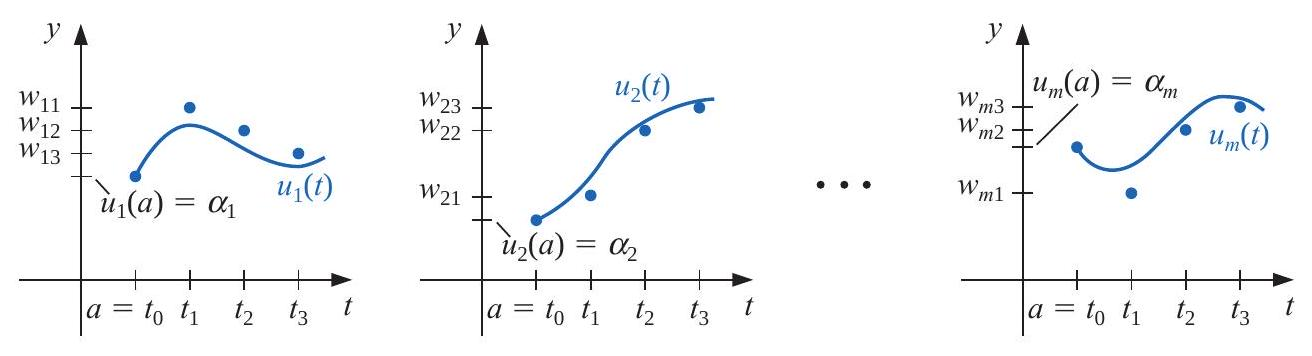
\includegraphics[width=14cmr]{2025_05_15_5266fa2c85d567bd073dg-72}
\caption{\scriptsize Figure $1$}
\label{fig:hoesdefig1}
\end{figure}

Suppose that the values $w_{1, j}, w_{2, j}, \ldots, w_{m, j}$ have been computed. We obtain $w_{1, j+1}$, $w_{2, j+1}, \ldots, w_{m, j+1}$ by first calculating


\begin{equation}\label{eqn:hoesdeeq5}
k_{1, i} =h f_{i}\left(t_{j}, w_{1, j}, w_{2, j}, \ldots, w_{m, j}\right), \quad \text { for each } i=1,2, \ldots, m 
\end{equation}

\begin{equation}\label{eqn:hoesdeeq6}
k_{2, i} =h f_{i}\left(t_{j}+\frac{h}{2}, w_{1, j}+\frac{1}{2} k_{1,1}, w_{2, j}+\frac{1}{2} k_{1,2}, \ldots, w_{m, j}+\frac{1}{2} k_{1, m}\right)
\end{equation}

for each $i=1,2, \ldots, m$;

\begin{equation}\label{eqn:hoesdeeq7}
k_{3, i}=h f_{i}\left(t_{j}+\frac{h}{2}, w_{1, j}+\frac{1}{2} k_{2,1}, w_{2, j}+\frac{1}{2} k_{2,2}, \ldots, w_{m, j}+\frac{1}{2} k_{2, m}\right) \tag{5.51}
\end{equation}

for each $i=1,2, \ldots, m$;

\begin{equation}\label{eqn:hoesdeeq8}
k_{4, i}=h f_{i}\left(t_{j}+h, w_{1, j}+k_{3,1}, w_{2, j}+k_{3,2}, \ldots, w_{m, j}+k_{3, m}\right)
\end{equation}

for each $i=1,2, \ldots, m$; and then

\begin{equation}\label{eqn:hoesdeeq9}
w_{i, j+1}=w_{i, j}+\frac{1}{6}\left(k_{1, i}+2 k_{2, i}+2 k_{3, i}+k_{4, i}\right)
\end{equation}

for each $i=1,2, \ldots, m$. Note that all the values $k_{1,1}, k_{1,2}, \ldots, k_{1, m}$ must be computed before any of the terms of the form $k_{2, i}$ can be determined. In general, each $k_{l, 1}, k_{l, 2}, \ldots, k_{l, m}$ must be computed before any of the expressions $k_{l+1, i}$.
%
%\section*{Runge-Kutta Method for Systems of Differential Equations}
%To approximate the solution of the $m$ th-order system of first-order initial-value problems
%
%$$
%u_{j}^{\prime}=f_{j}\left(t, u_{1}, u_{2}, \ldots, u_{m}\right), \quad a \leq t \leq b, \quad \text { with } \quad u_{j}(a)=\alpha_{j},
%$$
%
%for $j=1,2, \ldots, m$ at ( $N+1$ ) equally spaced numbers in the interval $[a, b]$ :
%
%INPUT endpoints $a, b$; number of equations $m$; integer $N$; initial conditions $\alpha_{1}, \ldots, \alpha_{m}$. OUTPUT approximations $w_{j}$ to $u_{j}(t)$ at the $(N+1)$ values of $t$.
%
%Step 1 Set $h=(b-a) / N$;
%
%$$
%t=a .
%$$
%
%Step 2 For $j=1,2, \ldots, m$ set $w_{j}=\alpha_{j}$.\\
%Step 3 OUTPUT $\left(t, w_{1}, w_{2}, \ldots, w_{m}\right)$.\\
%Step 4 For $i=1,2, \ldots, N$ do steps 5-11.\\
%Step 5 For $j=1,2, \ldots, m$ set
%
%$$
%k_{1, j}=h f_{j}\left(t, w_{1}, w_{2}, \ldots, w_{m}\right)
%$$
%
%Step 6 For $j=1,2, \ldots, m$ set
%
%$$
%k_{2, j}=h f_{j}\left(t+\frac{h}{2}, w_{1}+\frac{1}{2} k_{1,1}, w_{2}+\frac{1}{2} k_{1,2}, \ldots, w_{m}+\frac{1}{2} k_{1, m}\right) .
%$$
%
%Step 7 For $j=1,2, \ldots, m$ set
%
%$$
%k_{3, j}=h f_{j}\left(t+\frac{h}{2}, w_{1}+\frac{1}{2} k_{2,1}, w_{2}+\frac{1}{2} k_{2,2}, \ldots, w_{m}+\frac{1}{2} k_{2, m}\right) .
%$$
%
%Step 8 For $j=1,2, \ldots, m$ set
%
%$$
%k_{4, j}=h f_{j}\left(t+h, w_{1}+k_{3,1}, w_{2}+k_{3,2}, \ldots, w_{m}+k_{3, m}\right) .
%$$
%
%Step 9 For $j=1,2, \ldots, m$ set
%
%$$
%w_{j}=w_{j}+\left(k_{1, j}+2 k_{2, j}+2 k_{3, j}+k_{4, j}\right) / 6
%$$
%
%Step 10 Set $t=a+i h$.\\
%Step 11 OUTPUT $\left(t, w_{1}, w_{2}, \ldots, w_{m}\right)$.
%
%\section*{Step 12 STOP.}

\begin{example}
 Kirchhoff's Law states that the sum of all instantaneous voltage changes around a closed circuit is zero. This law implies that the current $I(t)$ in a closed circuit containing a resistance of $R$ ohms, a capacitance of $C$ farads, an inductance of $L$ henries, and a voltage source of $E(t)$ volts satisfies the equation

$$
L I^{\prime}(t)+R I(t)+\frac{1}{C} \int I(t) d t=E(t)
$$

The currents $I_{1}(t)$ and $I_{2}(t)$ in the left and right loops, respectively, of the circuit shown in Figure \ref{fig:hoesdefig2} are the solutions to the system of equations

$$
\begin{aligned}
2 I_{1}(t)+6\left[I_{1}(t)-I_{2}(t)\right]+2 I_{1}^{\prime}(t) & =12 \\
\frac{1}{0.5} \int I_{2}(t) d t+4 I_{2}(t)+6\left[I_{2}(t)-I_{1}(t)\right] & =0
\end{aligned}
$$

If the switch in the circuit is closed at time $t=0$, we have the initial conditions $I_{1}(0)=0$ and $I_{2}(0)=0$. Solve for $I_{1}^{\prime}(t)$ in the first equation, differentiate the second equation, and substitute for $I_{1}^{\prime}(t)$ to get

$$
\begin{aligned}
& I_{1}^{\prime}=f_{1}\left(t, I_{1}, I_{2}\right)=-4 I_{1}+3 I_{2}+6, \quad I_{1}(0)=0 \\
& I_{2}^{\prime}=f_{2}\left(t, I_{1}, I_{2}\right)=0.6 I_{1}^{\prime}-0.2 I_{2}=-2.4 I_{1}+1.6 I_{2}+3.6, \quad I_{2}(0)=0
\end{aligned}
$$

The exact solution to this system is

$$
\begin{aligned}
& I_{1}(t)=-3.375 e^{-2 t}+1.875 e^{-0.4 t}+1.5 \\
& I_{2}(t)=-2.25 e^{-2 t}+2.25 e^{-0.4 t}
\end{aligned}
$$

We will apply the Runge-Kutta method of order four to this system with $h=0.1$. Since $w_{1,0}=I_{1}(0)=0$ and $w_{2,0}=I_{2}(0)=0$,

$$
\begin{aligned}
k_{1,1} & =h f_{1}\left(t_{0}, w_{1,0}, w_{2,0}\right)=0.1 f_{1}(0,0,0)=0.1(-4(0)+3(0)+6)=0.6 \\
k_{1,2} & =h f_{2}\left(t_{0}, w_{1,0}, w_{2,0}\right)=0.1 f_{2}(0,0,0)=0.1(-2.4(0)+1.6(0)+3.6)=0.36 \\
k_{2,1} & =h f_{1}\left(t_{0}+\frac{1}{2} h, w_{1,0}+\frac{1}{2} k_{1,1}, w_{2,0}+\frac{1}{2} k_{1,2}\right)=0.1 f_{1}(0.05,0.3,0.18) \\
& =0.1(-4(0.3)+3(0.18)+6)=0.534 \\
k_{2,2} & =h f_{2}\left(t_{0}+\frac{1}{2} h, w_{1,0}+\frac{1}{2} k_{1,1}, w_{2,0}+\frac{1}{2} k_{1,2}\right)=0.1 f_{2}(0.05,0.3,0.18) \\
& =0.1(-2.4(0.3)+1.6(0.18)+3.6)=0.3168
\end{aligned}
$$

Generating the remaining entries in a similar manner produces

$$
\begin{aligned}
& k_{3,1}=(0.1) f_{1}(0.05,0.267,0.1584)=0.54072 \\
& k_{3,2}=(0.1) f_{2}(0.05,0.267,0.1584)=0.321264 \\
& k_{4,1}=(0.1) f_{1}(0.1,0.54072,0.321264)=0.4800912 \\
& k_{4,2}=(0.1) f_{2}(0.1,0.54072,0.321264)=0.28162944
\end{aligned}
$$

As a consequence,

$$
\begin{aligned}
I_{1}(0.1) \approx w_{1,1} & =w_{1,0}+\frac{1}{6}\left(k_{1,1}+2 k_{2,1}+2 k_{3,1}+k_{4,1}\right) \\
& =0+\frac{1}{6}(0.6+2(0.534)+2(0.54072)+0.4800912)=0.5382552
\end{aligned}
$$

and

$$
I_{2}(0.1) \approx w_{2,1}=w_{2,0}+\frac{1}{6}\left(k_{1,2}+2 k_{2,2}+2 k_{3,2}+k_{4,2}\right)=0.3196263
$$

The remaining entries in Table \ref{tab:hoesdetab1} are generated in a similar manner.
\end{example}

%Figure 5.7\\
\begin{figure}[h]
\centering
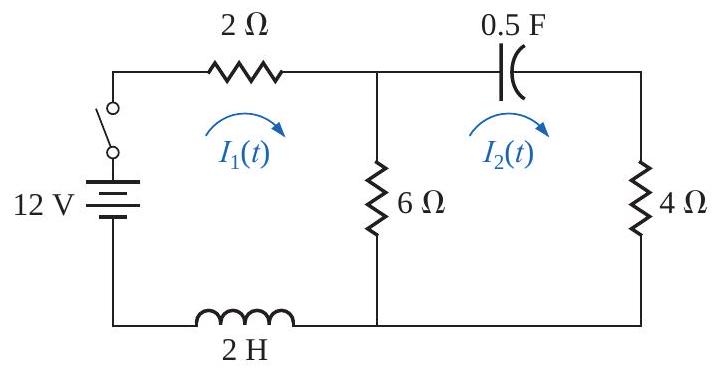
\includegraphics[width=9cm]{2025_05_15_5266fa2c85d567bd073dg-74}
\caption{\scriptsize Figure $2$}
\label{fig:hoesdefig2}
\end{figure}


%Table 5.19

\begin{table}[h]
\centering
\begin{tabular}{|l|l|l|l|l|}
\hline
$t_{j}$ & $w_{1, j}$ & $w_{2, j}$ & $\left|I_{1}\left(t_{j}\right)-w_{1, j}\right|$ & $\left|I_{2}\left(t_{j}\right)-w_{2, j}\right|$ \\
\hline
0.0 & 0 & 0 & 0 & 0 \\
\hline
0.1 & 0.5382550 & 0.3196263 & $0.8285 \times 10^{-5}$ & $0.5803 \times 10^{-5}$ \\
\hline
0.2 & 0.9684983 & 0.5687817 & $0.1514 \times 10^{-4}$ & $0.9596 \times 10^{-5}$ \\
\hline
0.3 & 1.310717 & 0.7607328 & $0.1907 \times 10^{-4}$ & $0.1216 \times 10^{-4}$ \\
\hline
0.4 & 1.581263 & 0.9063208 & $0.2098 \times 10^{-4}$ & $0.1311 \times 10^{-4}$ \\
\hline
0.5 & 1.793505 & 1.014402 & $0.2193 \times 10^{-4}$ & $0.1240 \times 10^{-4}$ \\
\hline
\end{tabular}
\caption{\scriptsize Table $4$}
\label{tab:hoesdetab1}
\end{table}

%Recall that Maple reserves the letter $D$ to represent differentiation.
%
%Maple's NumericalAnalysis package does not currently approximate the solution to systems of initial value problems, but systems of first-order differential equations can by solved using dsolve. The system in the Illustration is defined with\\
%sys $2:=D(u 1)(t)=-4 u 1(t)+3 u 2(t)+6, D(u 2)(t)=-2.4 u 1(t)+1.6 u 2(t)+3.6$\\
%and the initial conditions with\\
%init $2:=u 1(0)=0, u 2(0)=0$\\
%The system is solved with the command\\
%sol $2:=$ dsolve $(\{$ sys 2, init 2$\},\{u 1(t), u 2(t)\})$\\
%and Maple responds with
%
%$$
%\left\{u 1(t)=-\frac{27}{8} e^{-2 t}+\frac{15}{8} e^{-\frac{5}{2} t}+\frac{3}{2}, u 2(t)=-\frac{9}{4} e^{-2 t}+\frac{9}{4} e^{-\frac{5}{2} t}\right\}
%$$
%
%To isolate the individual functions we use\\
%$r 1:=\operatorname{rhs}(\operatorname{sol} 2[1]) ; r 2:=\operatorname{rhs}(\operatorname{sol} 2[2])$\\
%producing
%
%$$
%\begin{aligned}
%& -\frac{27}{8} e^{-2 t}+\frac{15}{8} e^{-\frac{5}{2} t}+\frac{3}{2} \\
%& -\frac{9}{4} e^{-2 t}+\frac{9}{4} e^{-\frac{5}{2} t}
%\end{aligned}
%$$
%
%and to determine the value of the functions at $t=0.5$ we use\\
%$\operatorname{evalf}(\operatorname{subs}(t=0.5, r 1)) ; \operatorname{evalf}(\operatorname{subs}(t=0.5, r 2))$\\
%giving, in agreement with Table 5.19,\\
%1.793527048\\
%1.014415451
%
%The command dsolve will fail if an explicit solution cannot be found. In that case we can use the numeric option in dsolve, which applies the Runge-Kutta-Fehlberg technique. This technique can also be used, of course, when the exact solution can be determined with dsolve. For example, with the system defined previously,\\
%$g:=$ dsolve (\{sys 2, init 2\}, \{ $u 1(t), u 2(t)\}$, numeric)\\
%returns
%
%$$
%\operatorname{proc}\left(x_{-} r k f 45\right) \ldots \text { end proc }
%$$
%
%To approximate the solutions at $t=0.5$, enter\\
%$g(0.5)$\\
%which gives approximations in the form
%
%$$
%[t=0.5, u 2(t)=1.014415563, u 1(t)=1.793527215]
%$$
%
\subsection*{Higher-Order Differential Equations}
%Many important physical problems-for example, electrical circuits and vibrating systemsinvolve initial-value problems whose equations have orders higher than one. New techniques are not required for solving these problems. By relabeling the variables, we can reduce a higher-order differential equation into a system of first-order differential equations and then apply one of the methods we have already discussed.

A general $m$ th-order initial-value problem

$$
y^{(m)}(t)=f\left(t, y, y^{\prime}, \ldots, y^{(m-1)}\right), \quad a \leq t \leq b
$$

with initial conditions $y(a)=\alpha_{1}, y^{\prime}(a)=\alpha_{2}, \ldots, y^{(m-1)}(a)=\alpha_{m}$ can be converted into a system of equations in the form (5.45) and (5.46).

Let $u_{1}(t)=y(t), u_{2}(t)=y^{\prime}(t), \ldots$, and $u_{m}(t)=y^{(m-1)}(t)$. This produces the first-order system

$$
\frac{d u_{1}}{d t}=\frac{d y}{d t}=u_{2}, \quad \frac{d u_{2}}{d t}=\frac{d y^{\prime}}{d t}=u_{3}, \quad \cdots, \quad \frac{d u_{m-1}}{d t}=\frac{d y^{(m-2)}}{d t}=u_{m}
$$

and

$$
\frac{d u_{m}}{d t}=\frac{d y^{(m-1)}}{d t}=y^{(m)}=f\left(t, y, y^{\prime}, \ldots, y^{(m-1)}\right)=f\left(t, u_{1}, u_{2}, \ldots, u_{m}\right)
$$

with initial conditions

$$
u_{1}(a)=y(a)=\alpha_{1}, \quad u_{2}(a)=y^{\prime}(a)=\alpha_{2}, \quad \ldots, \quad u_{m}(a)=y^{(m-1)}(a)=\alpha_{m}
$$

\begin{example}
Transform the the second-order initial-value problem

$$
y^{\prime \prime}-2 y^{\prime}+2 y=e^{2 t} \sin t, \quad \text { for } 0 \leq t \leq 1, \quad \text { with } y(0)=-0.4, y^{\prime}(0)=-0.6
$$

into a system of first order initial-value problems, and use the Runge-Kutta method with $h=0.1$ to approximate the solution.
\end{example}

\begin{mysolution}
Let $u_{1}(t)=y(t)$ and $u_{2}(t)=y^{\prime}(t)$. This transforms the second-order equation into the system

$$
\begin{aligned}
& u_{1}^{\prime}(t)=u_{2}(t) \\
& u_{2}^{\prime}(t)=e^{2 t} \sin t-2 u_{1}(t)+2 u_{2}(t)
\end{aligned}
$$

with initial conditions $u_{1}(0)=-0.4, u_{2}(0)=-0.6$.\\
The initial conditions give $w_{1,0}=-0.4$ and $w_{2,0}=-0.6$. The Runge-Kutta Eqs. (5.49) through (5.52) on page 330 with $j=0$ give

$$
\begin{aligned}
k_{1,1} & =h f_{1}\left(t_{0}, w_{1,0}, w_{2,0}\right)=h w_{2,0}=-0.06 \\
k_{1,2} & =h f_{2}\left(t_{0}, w_{1,0}, w_{2,0}\right)=h\left[e^{2 t_{0}} \sin t_{0}-2 w_{1,0}+2 w_{2,0}\right]=-0.04 \\
k_{2,1} & =h f_{1}\left(t_{0}+\frac{h}{2}, w_{1,0}+\frac{1}{2} k_{1,1}, w_{2,0}+\frac{1}{2} k_{1,2}\right)=h\left[w_{2,0}+\frac{1}{2} k_{1,2}\right]=-0.062 \\
k_{2,2} & =h f_{2}\left(t_{0}+\frac{h}{2}, w_{1,0}+\frac{1}{2} k_{1,1}, w_{2,0}+\frac{1}{2} k_{1,2}\right) \\
& =h\left[e^{2\left(t_{0}+0.05\right)} \sin \left(t_{0}+0.05\right)-2\left(w_{1,0}+\frac{1}{2} k_{1,1}\right)+2\left(w_{2,0}+\frac{1}{2} k_{1,2}\right)\right] \\
& =-0.03247644757 \\
k_{3,1} & =h\left[w_{2,0}+\frac{1}{2} k_{2,2}\right]=-0.06162832238 \\
k_{3,2} & =h\left[e^{2\left(t_{0}+0.05\right)} \sin \left(t_{0}+0.05\right)-2\left(w_{1,0}+\frac{1}{2} k_{2,1}\right)+2\left(w_{2,0}+\frac{1}{2} k_{2,2}\right)\right] \\
& =-0.03152409237 \\
k_{4,1} & =h\left[w_{2,0}+k_{3,2}\right]=-0.06315240924
\end{aligned}
$$

and

$$
k_{4,2}=h\left[e^{2\left(t_{0}+0.1\right)} \sin \left(t_{0}+0.1\right)-2\left(w_{1,0}+k_{3,1}\right)+2\left(w_{2,0}+k_{3,2}\right)\right]=-0.02178637298
$$

So

$$
w_{1,1}=w_{1,0}+\frac{1}{6}\left(k_{1,1}+2 k_{2,1}+2 k_{3,1}+k_{4,1}\right)=-0.4617333423
$$

and

$$
w_{2,1}=w_{2,0}+\frac{1}{6}\left(k_{1,2}+2 k_{2,2}+2 k_{3,2}+k_{4,2}\right)=-0.6316312421
$$

The value $w_{1,1}$ approximates $u_{1}(0.1)=y(0.1)=0.2 e^{2(0.1)}(\sin 0.1-2 \cos 0.1)$, and $w_{2,1}$ approximates $u_{2}(0.1)=y^{\prime}(0.1)=0.2 e^{2(0.1)}(4 \sin 0.1-3 \cos 0.1)$.

The set of values $w_{1, j}$ and $w_{2, j}$, for $j=0,1, \ldots, 10$, are presented in Table \ref{tab:hoesdetab1} and are compared to the actual values of $u_{1}(t)=0.2 e^{2 t}(\sin t-2 \cos t)$ and $u_{2}(t)=u_{1}^{\prime}(t)=$ $0.2 e^{2 t}(4 \sin t-3 \cos t)$.
\end{mysolution}
%Table 5.20

\begin{table}[h]
\centering
\begin{tabular}{|l|l|l|l|l|l|l|}
\hline
$t_{j}$ & $y\left(t_{j}\right)=u_{1}\left(t_{j}\right)$ & $w_{1, j}$ & $y^{\prime}\left(t_{j}\right)=u_{2}\left(t_{j}\right)$ & $w_{2, j}$ & $\left|y\left(t_{j}\right)-w_{1, j}\right|$ & $\left|y^{\prime}\left(t_{j}\right)-w_{2, j}\right|$ \\
\hline
0.0 & -0.40000000 & -0.40000000 & -0.6000000 & -0.60000000 & 0 & 0 \\
\hline
0.1 & -0.46173297 & -0.46173334 & -0.6316304 & -0.63163124 & $3.7 \times 10^{-7}$ & $7.75 \times 10^{-7}$ \\
\hline
0.2 & -0.52555905 & -0.52555988 & -0.6401478 & -0.64014895 & $8.3 \times 10^{-7}$ & $1.01 \times 10^{-6}$ \\
\hline
0.3 & -0.58860005 & -0.58860144 & -0.6136630 & -0.61366381 & $1.39 \times 10^{-6}$ & $8.34 \times 10^{-7}$ \\
\hline
0.4 & -0.64661028 & -0.64661231 & -0.5365821 & -0.53658203 & $2.03 \times 10^{-6}$ & $1.79 \times 10^{-7}$ \\
\hline
0.5 & -0.69356395 & -0.69356666 & -0.3887395 & -0.38873810 & $2.71 \times 10^{-6}$ & $5.96 \times 10^{-7}$ \\
\hline
0.6 & -0.72114849 & -0.72115190 & -0.1443834 & -0.14438087 & $3.41 \times 10^{-6}$ & $7.75 \times 10^{-7}$ \\
\hline
0.7 & -0.71814890 & -0.71815295 & 0.2289917 & 0.22899702 & $4.05 \times 10^{-6}$ & $2.03 \times 10^{-6}$ \\
\hline
0.8 & -0.66970677 & -0.66971133 & 0.7719815 & 0.77199180 & $4.56 \times 10^{-6}$ & $5.30 \times 10^{-6}$ \\
\hline
0.9 & -0.55643814 & -0.55644290 & 1.534764 & 1.5347815 & $4.76 \times 10^{-6}$ & $9.54 \times 10^{-6}$ \\
\hline
1.0 & -0.35339436 & -0.35339886 & 2.578741 & 2.5787663 & $4.50 \times 10^{-6}$ & $1.34 \times 10^{-5}$ \\
\hline
\end{tabular}
\caption{\scriptsize Table $5$}
\label{tab:hoesdetab2}
\end{table}

%In Maple the $n$th derivative $y^{(n)}(t)$ is specified by $(D @ @ n)(y)(t)$.
%
%We can also use dsolve from Maple on higher-order equations. To define the differential equation in Example 1, use\\
%$\operatorname{def} 2:=(D @ @ 2)(y)(t)-2 D(y)(t)+2 y(t)=e^{2 t} \sin (t)$\\
%and to specify the initial conditions use\\
%init $2:=y(0)=-0.4, D(y)(0)=-0.6$\\
%The solution is obtained with the command\\
%sol $2:=$ dsolve $(\{$ def 2, init 2$\}, y(t))$\\
%to obtain
%
%$$
%y(t)=\frac{1}{5} e^{2 t}(\sin (t)-2 \cos (t))
%$$
%
%We isolate the solution in function form using\\
%$g:=\operatorname{rhs}(\operatorname{sol} 2)$\\
%To obtain $y(1.0)=g(1.0)$, enter\\
%$\operatorname{evalf}(\operatorname{subs}(t=1.0, g))$\\
%which gives -0.3533943574 .\\
Runge-Kutta-Fehlberg is also available for higher-order equations via the dsolve command with the numeric option. It is employed in the same manner as illustrated for systems of equations.

The other one-step methods can be extended to systems in a similar way. When error control methods like the Runge-Kutta-Fehlberg method are extended, each component of the numerical solution $\left(w_{1 j}, w_{2 j}, \ldots, w_{m j}\right)$ must be examined for accuracy. If any of the components fail to be sufficiently accurate, the entire numerical solution $\left(w_{1 j}, w_{2 j}, \ldots, w_{m j}\right)$ must be recomputed.

The multistep methods and predictor-corrector techniques can also be extended to systems. Again, if error control is used, each component must be accurate. The extension of the extrapolation technique to systems can also be done, but the notation becomes quite involved. 

%Convergence theorems and error estimates for systems are similar to those considered in Section 5.10 for the single equations, except that the bounds are given in terms of vector norms, a topic considered in Chapter 7. (A good reference for these theorems is [Ge1], pp. 45-72.)

\begin{myexercise}%\label{Comprehensionquiz2}
Use the Runge-Kutta for Systems Algorithm to approximate the solutions of the following higher order differential equations, and compare the results to the actual solutions.
\begin{enumerate}[label=(\alph*)]
\item $y^{\prime \prime}-2 y^{\prime}+y=t e^{t}-t$, $0 \leq t \leq 1$, $y(0)=y^{\prime}(0)=0$, with $h=0.1$;
actual solution $y(t)=\frac{1}{6} t^{3} e^{t}-t e^{t}+2 e^{t}-t-2$.\\
\item $t^{2} y^{\prime \prime}-2 t y^{\prime}+2 y=t^{3} \ln t$, $1 \leq t \leq 2, \quad y(1)=1$, $y^{\prime}(1)=0$, with $h=0.1$; actual solution $y(t)=\frac{7}{4} t+\frac{1}{2} t^{3} \ln t-\frac{3}{4} t^{3}$.
%\item $y^{\prime \prime \prime}+2 y^{\prime \prime}-y^{\prime}-2 y=e^{t}$, $0 \leq t \leq 3, \quad y(0)=1$, $y^{\prime}(0)=2$, $y^{\prime \prime}(0)=0$, with $h=0.2$; actual solution $y(t)=\frac{43}{36} e^{t}+\frac{1}{4} e^{-t}-\frac{4}{9} e^{-2 t}+\frac{1}{6} t e^{t}$.\\
%\item $t^{3} y^{\prime \prime \prime}-t^{2} y^{\prime \prime}+3 t y^{\prime}-4 y=5 t^{3} \ln t+9 t^{3}$, $1 \leq t \leq 2$, $y(1)=0, \quad y^{\prime}(1)=1$, $y^{\prime \prime}(1)=3$, with $h=0.1$; actual solution $y(t)=-t^{2}+t \cos (\ln t)+t \sin (\ln t)+t^{3} \ln t$.
\end{enumerate}

\begin{mysolution}
The Runge-Kutta for Systems Algorithm gives the results in the following tables.\\
\begin{enumerate}[label=(\alph*).]
\item

\begin{center}
\begin{tabular}{ccc}
\hline
$t_{i}$ & $w_{1 i}$ & $y_{i}$ \\
\hline
0.200 & 0.00015352 & 0.00015350 \\
0.500 & 0.00742968 & 0.00743027 \\
0.700 & 0.03299617 & 0.03299805 \\
1.000 & 0.17132224 & 0.17132880 \\
\hline
\end{tabular}
\end{center}

\item
\begin{center}
\begin{tabular}{ccc}
\hline
$t_{i}$ & $w_{1 i}$ & $y_{i}$ \\
\hline
1.200 & 0.96152437 & 0.96152583 \\
1.500 & 0.77796897 & 0.77797237 \\
1.700 & 0.59373369 & 0.59373830 \\
2.000 & 0.27258237 & 0.27258872 \\
\end{tabular}
\end{center}


%\item
%
%\begin{center}
%\begin{tabular}{ccc}
%\hline
%$t_{i}$ & $w_{1 i}$ & $y_{i}$ \\
%\hline
%1.000 & 3.73162695 & 3.73170445 \\
%2.000 & 11.31424573 & 11.31452924 \\
%3.000 & 34.04395688 & 34.04517155 \\
%\hline
%\end{tabular}
%\end{center}
%
%\item
%
%\begin{center}
%\begin{tabular}{ccc}
%\hline
%$t_{i}$ & $w_{1 i}$ & $w_{2 i}$ \\
%\hline
%1.200 & 0.27273759 & 0.27273791 \\
%1.500 & 1.08849079 & 1.08849259 \\
%1.700 & 2.04353207 & 2.04353642 \\
%2.000 & 4.36156675 & 4.36157780 \\
%\hline
%\end{tabular}
%\end{center}

\end{enumerate}
\end{mysolution}
\end{myexercise}





\section{Stability and Stiff Differential Equations}
%\videolesson
%\begin{selfvideo}[2]
%%LESSON 3: 
%This video presents a discussion on stability and stiff differential equations. Follow the discussion and then solve the problems in the subsequent quiz.
%\end{selfvideo}
%\begin{boxB}Question: \end{boxB}

\begin{youtube}
This video presents a discussion on stability and stiff differential equations. Follow the discussion and then solve the problems in the subsequent quiz.
\end{youtube}

\mylink{https://www.youtube.com/watch?\\v=yABmV2qnzcg\&list=PLkiPLxr5Ckwsk1A\_qK\_AK\_8LGFoxqdox2\&index=5}

\mylink{https://www.youtube.com/watch?v=-YoojEp24BA}

\mylink{https://www.youtube.com/watch?v=lQENz3-HOLQ}

\mylink{https://www.youtube.com/watch?v=C72rIeiv7mg}
\begin{myexercise}%\label{Comprehensionquiz2}
Given the multistep method

$$
w_{i+1}=-\frac{3}{2} w_{i}+3 w_{i-1}-\frac{1}{2} w_{i-2}+3 h f\left(t_{i}, w_{i}\right), \quad \text { for } i=2, \ldots, N-1,
$$

with starting values $w_{0}, w_{1}, w_{2}$ :
\begin{enumerate}[label=(\alph*)]
\item  Find the local truncation error.
\item Comment on consistency, stability, and convergence.
\end{enumerate}

\begin{mysolution}


\begin{enumerate}[label=(\alph*)]
\item The local truncation error is $\tau_{i+1}=\frac{1}{4} h^{3} y^{(4)}\left(\xi_{i}\right)$, for some $\xi$, where $t_{i-2}<\xi_{i}<t_{i+1}$.\\
\item The method is consistent but unstable and not convergent.
\end{enumerate}
\end{mysolution}
\end{myexercise}


%\discussion


\begin{posttest}%[\textcolor{red}{End of Module 8 Quiz}]
\item An electrical circuit consists of a capacitor of constant capacitance $C=1.1$ farads in series with a resistor of constant resistance $R_{0}=2.1$ ohms. A voltage $\mathcal{E}(t)=110 \sin t$ is applied at time $t=0$. When the resistor heats up, the resistance becomes a function of the current $i$,


$$
R(t)=R_{0}+k i, \quad \text { where } k=0.9
$$

and the differential equation for $i(t)$ becomes

$$
\left(1+\frac{2 k}{R_{0}} i\right) \frac{d i}{d t}+\frac{1}{R_{0} C} i=\frac{1}{R_{0} C} \frac{d \mathcal{E}}{d t}
$$

Find $i(2)$, assuming that $i(0)=0$. 


\item Use the Extrapolation Algorithm with tolerance $T O L=10^{-6}, h \max =0.5$, and $h \min =0.05$ to approximate the solutions to the following initial-value problems. Compare the results to the actual values.
\begin{enumerate}[label=(\alph*)]
  \item $\quad y^{\prime}=y / t-(y / t)^{2}, \quad 1 \leq t \leq 4, \quad y(1)=1$; actual solution $y(t)=t /(1+\ln t)$.\\
\item $\quad y^{\prime}=1+y / t+(y / t)^{2}, \quad 1 \leq t \leq 3, \quad y(1)=0$; actual solution $y(t)=t \tan (\ln t)$.
\end{enumerate}

\item Use the Runge-Kutta for Systems Algorithm to approximate the solutions of the following higher order differential equations, and compare the results to the actual solutions.
\begin{enumerate}[label=(\alph*)]
%\item $y^{\prime \prime}-2 y^{\prime}+y=t e^{t}-t$, $0 \leq t \leq 1$, $y(0)=y^{\prime}(0)=0$, with $h=0.1$;
%actual solution $y(t)=\frac{1}{6} t^{3} e^{t}-t e^{t}+2 e^{t}-t-2$.\\
%\item $t^{2} y^{\prime \prime}-2 t y^{\prime}+2 y=t^{3} \ln t$, $1 \leq t \leq 2, \quad y(1)=1$, $y^{\prime}(1)=0$, with $h=0.1$; actual solution $y(t)=\frac{7}{4} t+\frac{1}{2} t^{3} \ln t-\frac{3}{4} t^{3}$.\\
\item $y^{\prime \prime \prime}+2 y^{\prime \prime}-y^{\prime}-2 y=e^{t}$, $0 \leq t \leq 3, \quad y(0)=1$, $y^{\prime}(0)=2$, $y^{\prime \prime}(0)=0$, with $h=0.2$; actual solution $y(t)=\frac{43}{36} e^{t}+\frac{1}{4} e^{-t}-\frac{4}{9} e^{-2 t}+\frac{1}{6} t e^{t}$.\\
\item $t^{3} y^{\prime \prime \prime}-t^{2} y^{\prime \prime}+3 t y^{\prime}-4 y=5 t^{3} \ln t+9 t^{3}$, $1 \leq t \leq 2$, $y(1)=0, \quad y^{\prime}(1)=1$, $y^{\prime \prime}(1)=3$, with $h=0.1$; actual solution $y(t)=-t^{2}+t \cos (\ln t)+t \sin (\ln t)+t^{3} \ln t$.
\end{enumerate}

\item Solve the following stiff initial-value problem using the Runge-Kutta fourth-order method with (a) $h=0.1$ and (b) $h=0.025$.


$$
\begin{aligned}
& u_{1}^{\prime}=32 u_{1}+66 u_{2}+\frac{2}{3} t+\frac{2}{3}, \quad 0 \leq t \leq 0.5, \quad u_{1}(0)=\frac{1}{3} \\
& u_{2}^{\prime}=-66 u_{1}-133 u_{2}-\frac{1}{3} t-\frac{1}{3}, \quad 0 \leq t \leq 0.5, \quad u_{2}(0)=\frac{1}{3}
\end{aligned}
$$

Compare the results to the actual solution,

$$
u_{1}(t)=\frac{2}{3} t+\frac{2}{3} e^{-t}-\frac{1}{3} e^{-100 t} \quad \text { and } \quad u_{2}(t)=-\frac{1}{3} t-\frac{1}{3} e^{-t}+\frac{2}{3} e^{-100 t}
$$

\begin{mysolution}
\begin{enumerate}[label=\arabic*.]
  \item The current after 2 seconds is approximately $i(2)=8.693$ amperes.

\item The Extrapolation Algorithm gives the results in the following tables.\\
\begin{enumerate}[label=(\alph*).]
\item

\begin{center}
\begin{tabular}{cccccc}
\hline
$i$ & $t_{i}$ & $w_{i}$ & $h$ & $k$ & $y_{i}$ \\
\hline
1 & 1.50 & 1.06726237 & 0.50 & 4 & 1.06726235 \\
2 & 2.00 & 1.18123223 & 0.50 & 3 & 1.18123222 \\
3 & 2.50 & 1.30460372 & 0.50 & 3 & 1.30460371 \\
4 & 3.00 & 1.42951608 & 0.50 & 3 & 1.42951607 \\
5 & 3.50 & 1.55364771 & 0.50 & 3 & 1.55364770 \\
6 & 4.00 & 1.67623915 & 0.50 & 3 & 1.67623914 \\
\hline
\end{tabular}
\end{center}

\item

\begin{center}
\begin{tabular}{cccccc}
\hline
$i$ & $t_{i}$ & $w_{i}$ & $h$ & $k$ & $y_{i}$ \\
\hline
1 & 1.50 & 0.64387537 & 0.50 & 4 & 0.64387533 \\
2 & 2.00 & 1.66128182 & 0.50 & 5 & 1.66128176 \\
3 & 2.50 & 3.25801550 & 0.50 & 5 & 3.25801536 \\
4 & 3.00 & 5.87410027 & 0.50 & 5 & 5.87409998 \\
\hline
\end{tabular}
\end{center}
\end{enumerate}

\vspace{5mm}
\item The Runge-Kutta for Systems Algorithm gives the results in the following tables.\\
\begin{enumerate}[label=(\alph*).]
\item

\begin{center}
\begin{tabular}{ccc}
\hline
$t_{i}$ & $w_{1 i}$ & $y_{i}$ \\
\hline
1.000 & 3.73162695 & 3.73170445 \\
2.000 & 11.31424573 & 11.31452924 \\
3.000 & 34.04395688 & 34.04517155 \\
\hline
\end{tabular}
\end{center}

\item

\begin{center}
\begin{tabular}{ccc}
\hline
$t_{i}$ & $w_{1 i}$ & $w_{2 i}$ \\
\hline
1.200 & 0.27273759 & 0.27273791 \\
1.500 & 1.08849079 & 1.08849259 \\
1.700 & 2.04353207 & 2.04353642 \\
2.000 & 4.36156675 & 4.36157780 \\
\hline
\end{tabular}
\end{center}

\end{enumerate}

\vspace{5mm}
\item 
\begin{enumerate}[label=(\alph*).]
\item
\begin{center}
\begin{tabular}{|l|l|l|l|l|}
\hline
$t_{i}$ & $w_{1 i}$ & $u_{1 i}$ & $w_{2 i}$ & $u_{2 i}$ \\
\hline
0.100 & -96.33011 & 0.66987648 & 193.6651 & -0.33491554 \\
\hline
0.200 & -28226.32 & 0.67915383 & 56453.66 & -0.33957692 \\
\hline
0.300 & -8214056 & 0.69387881 & 16428113 & -0.34693941 \\
\hline
0.400 & -2390290586 & 0.71354670 & 4780581173 & -0.35677335 \\
\hline
0.500 & -695574560790 & 0.73768711 & 1391149121600 & -0.36884355 \\
\hline
\end{tabular}
\end{center}

\item

\begin{center}
\begin{tabular}{ccccc}
\hline
$t_{i}$ & $w_{1 i}$ & $u_{1 i}$ & $w_{2 i}$ & $u_{2 i}$ \\
\hline
0.100 & 0.61095960 & 0.66987648 & -0.21708179 & -0.33491554 \\
0.200 & 0.66873489 & 0.67915383 & -0.31873903 & -0.33957692 \\
0.300 & 0.69203679 & 0.69387881 & -0.34325535 & -0.34693941 \\
0.400 & 0.71322103 & 0.71354670 & -0.35612202 & -0.35677335 \\
0.500 & 0.73762953 & 0.73768711 & -0.36872840 & -0.36884355 \\
\hline
\end{tabular}
\end{center}
\end{enumerate}
\end{enumerate}
\end{mysolution}
\end{posttest}

%share your understanding of properties of functions and their applications to solving rates of change problems in physical phenomenon 


%\end{actsoln}

\takehome

\comy{You are now at the last part of this module. Your  task is to do a self-reflection on your learning experience.}



\references
\begin{refenumerate}
\item Kong, Q., Siauw, T., Bayen, A., (2020). Python Programming and Numerical Methods. First Edition, Academic Press,  ISBN-13 ‏ : ‎ 978-0128195499 \\
\mylink{https://pythonnumericalmethods.studentorg.berkeley.edu/notebooks/Index.html}
%chapter 1 pg 7-36 functions\\
%chapter 1 pg 51-83 limits and continuity\\
%chapter 1 pg 45-50 rates of change\\
%chapter 2 pg 108-120 the derivative\\
%\item Mendelson, E. (2022). Schaum's Outline of Calculus. McGraw-Hill Education.
%chapter 6 51-55 functions
%chapter 7 59-65 limits
%chapter 8 69-74 continuity
%chapter 9 77-81 derivative
%\item Calculus \mylink{https://math.libretexts.org/Bookshelves/Calculus}
%\item Chris McMullen, 2021, Essential Calculus Skills Practice Workbook with Full Solutions, Zishka Publishing, ISBN 978-1-941691-24-3
%\item R. Adams and C. Essex, 2021, Calculus: A complete Course, Addison Wesley, ISBN 13: 978-0135732588
%\item P. Abbott and H. Neill, 2018, Calculus: A Complete Introduction: The Easy Way to Learn Calculus (Teach Yourself), ISBN 13: 978-1473678446
\end{refenumerate}





%\wrapup
%To wrap-up, answer the following questions:
%
%\begin{enumerate}
%\item 
%%when do we say that a limit of a function exists?
%%\item how do we remove discontinuity in functions?
%%\item what is the relationship between the gradient of the tangent line and the derivative?
%\end{enumerate}
















%\newpage

%\facilitation


%
\begin{center}
    {\Large \textbf{FUNCTIONS OF SEVERAL VARIABLES}}\\[2mm]
(DEFINITION, DOMAIN, RANGE, GRAPHS AND LEVEL CURVES) \\[4mm]

\mycenterbox{5 minute review}%\\[4mm]
Recap the definition of a function of several variables, and the meaning of domain, range, graph and level curves of functions of several variables.
\end{center}
\mycenterbox{Warm-up.}%\\[4mm]
\problemAnswer{
Match the function with its graph (labeled I–VI).Give reasons for your choices
\begin{multicols}{3}
\begin{enumerate}[label=(\alph*)]
\item $f(x,y)=|x|+|y|$\\[4mm]
\item $f(x,y)=|xy|$
\item $f(x,y)=\frac{1}{1+x^2+y^2}$\\2mm]
\item $f(x,y)=(x^2-y^2)^2$
\item $f(x,y)=(x-y)^2$\\[4mm]
\item $f(x,y)=\sin(|x|+|y|)$
\end{enumerate}
\end{multicols}

\begin{center}
%\centering
\includegraphics[width=10cm]{MCTutorial1Q1.JPEG}
\end{center}
%\tcbox[tcbox raise base]{Warm-up}
 
%\begin{flushright}
%\begin{tikzpicture}
%    % A body
%
%
%    % Non-rectangle shapes must be drawn as polygone
%    \begin{scope}[shift={(3,0)}]
%        \draw  (0,0.5) -- (0,4) -- (.5,4) -- (.5,4.5) -- (1.,4.5) -- (4.,4.5) --(4.,4)-- (4.5,4) --(4.5,0.5) --(4.0,0.5)--(4.0,0.0)-- (.5,0) --(0.5,0.5) -- cycle;
%        % Draw symmetry lines
%        \draw [symmetry] (.5, 0.5) -- (.5,4.0);
%        \draw [symmetry] (4, 0.5) -- (4,4.0);
%        \draw [symmetry] (.5,4.0) -- (4,4.0);
%         \draw [symmetry] (.5, 0.5) -- (4, 0.5);
%        % Dimensions
%        \draw (4.5,0) -- ++(0.5,0) coordinate (D1) -- +(5pt,0);
%        \draw (4.5,4.5) -- ++(0.5,0) coordinate (D2) -- +(5pt,0);
%        \draw [dimen] (D1) -- (D2) node {6cm};
%       
%        
%        \draw (0.0,5) -- ++(0,0.5) coordinate (D1) -- +(0,+5pt);
%        \draw (0.5,5) -- ++(0,0.5) coordinate (D2) -- +(0,+5pt);
%        \draw [dimen,-] (D1) -- (D2) node [above=5pt] {$x$ cm};
%        \draw [dimen,<-] (D1) -- ++(-5pt,0);
%        \draw [dimen,<-] (D2) -- ++(+5pt,0);
%    \end{scope}
%\end{tikzpicture}
%\end{flushright}

}


\mycenterbox{Problems.}%

%\begin{center}
%\tcbox[tcbox raise base]{ Problems. Choose from the below}
%\end{center}
\problem{Exploring functions}%
\begin{enumerate}[(a)]
\item Are the following functions even, odd, or neither? What can you say
about their range?
\begin{multicols}{4}
 \begin{enumerate}[(i)]
\item $\displaystyle \frac{3x}{x^2+2}$
\item $\displaystyle \cos x+3$
\item $\displaystyle \frac{2x^3}{\cos x+3}$
\item $\displaystyle \frac{3x^4+2x^2}{\sin x+4}$
\end{enumerate}
\end{multicols}
\item Consider the functions $\sin^n x$ and $\cos^n x$, where $n$ is a positive integer.
Which are odd, which are even, and what are their periodicities?
\item What is the periodicity of $f(x) = 2 \cos x+\sin 2x$? Is it even/odd/neither?

\end{enumerate}

\problem{Cubic functions} 
Show that $x-1$ is a factor of the cubic function%
$$P(x)=x^3-2x^2-5x+6,$$
and  find the quadratic factor $Q(x)$ such that $P(x) = (x -1)Q(x)$. Factorise
$Q(x)$ and hence sketch $P(x).$

%\newpage
\problem{Sigmoid functions*.}%
For positive integers $n$, consider the family of functions
$$\displaystyle f_n= \frac{x^n}{2^n+x^n}.$$
\begin{enumerate}[(a)]
\item What are appropriate domains and ranges for $f_n(x)$? Do they depend on $n$?

\item Is $f_n(x)$ even, odd, or neither? Does this depend on $n$?

\item Show that for $x\geq 0$, $f_n(x)$ are strictly increasing functions and that
$0\leq f_n(x) < 1.$
\item What is the value of $f_n(2)$? Does it depend on $n$?

\item By considering the values of $f_n(1.9)$ and $f_n(2.1)$ for $n = 2, 4, 8, 16, 32$ and
$64$, show that the graph of $f_n(x)$ for $x\ge 0$ is an increasing sigmoid (that
is, $S$-shaped) function that approaches a step function as $n\rightarrow \infty$.
\end{enumerate}

\mycenterbox{Selected answers and hints}%

For the warm-up, $V(x)=4x(3-x)^2$. Writing $x=1+\epsilon$, we get
$$V = 4(1 +\epsilon)(3- (1+\epsilon))^2=4(4-\epsilon^2(3-\epsilon)).$$
If $-1<\epsilon<2$ then $\epsilon^2 (3-\epsilon)\ge 0$, with equality when $\epsilon=0$. Thus the maximum
value of $V$ occurs when $\epsilon= 0$, i.e. $x = 1\rm{cm}$.

\begin{enumerate}
\item 
\begin{enumerate}[(i)]
\item Odd. The range is the interval  $[-\frac{3}{4}\sqrt{2},\; \frac{3}{4}\sqrt{2}]$
\item Even. The range is the interval $[2, 4]$.
\item Odd. The range is all of $\mathbb R$.
\item Neither. (For example, writing $\displaystyle \frac{5}{\sin x+4}$ we have $\displaystyle f(1)= \frac{5}{\sin (1)+4} \equiv 1.032 (3\rm{dp})$ which is neither $f(1)$ nor $-f(1)$.)\\[4mm]
The range is the nonnegative reals $[0,\infty)$

\end{enumerate}
\end{enumerate}










